\chapter{Grundlagen von Apache Hadoop\textsuperscript{\textregistered}}
\label{ch:theory_hadoop}

\section{Apache Hadoop Framework}
\label{sec:theory_hadoop}
\noindent
Apache Hadoop\textsuperscript{\textregistered} ist ein etabliertes Java-Framework zur verteilten Speicherung und Verarbeitung von Daten. Durch die parallele Ausführung von Algorithmen, eignet sich ein Hadoop-Cluster für rechenaufwendige Datenanalysen. Ein primäres Paradigma ist das Konzept der \textit{Datenlokalität}. Die auszuführenden Programme werden auf die Knoten verteilt, auf welchen auch die Daten liegen. Ressourcenintensive Datentransporte sollen weitgehend vermieden werden.\cite[S. 20 ff.]{big_data_praxis}\\ 
Das Framework ist für die Ausführung auf Standardhardware konzipiert. Es wird also keine verhältnismäßig teure Spezialhardware benötigt. Das Cluster besteht aus vielen einzelnen Knoten mit Standardcomputern, welche im Verhältnis zu Spezialservern günstiger und leicht ersetzbar sind. Der Ausfall einzelner Knoten wird bei der Datenhaltung entsprechend berücksichtigt. \\

\noindent
Hadoop selbst besteht aus mehreren Komponenten, welche spezifische Aufgaben übernehmen. Abbildung \ref{fig:hadoop_framework_structure} stellt eine grobe Skizzierung der Komponentenlandschaft der Plattform dar.\footnote{In der Abbildung \ref{fig:hadoop_framework_structure} werden Logos der einzelnen Apache Projekte verwendet. Diese sind Handelsmarken der \textit{Apache Source Foundation} (siehe Link: \url{https://www.apache.org/}. Letzter Zugriff: 6.10.2018). In Kapitel \ref{sec:licencing_issues} im Anhang werden die Logos und deren Herkunft nochmals aufgelistet.}\\

\begin{figure}[ht]
  \centering
  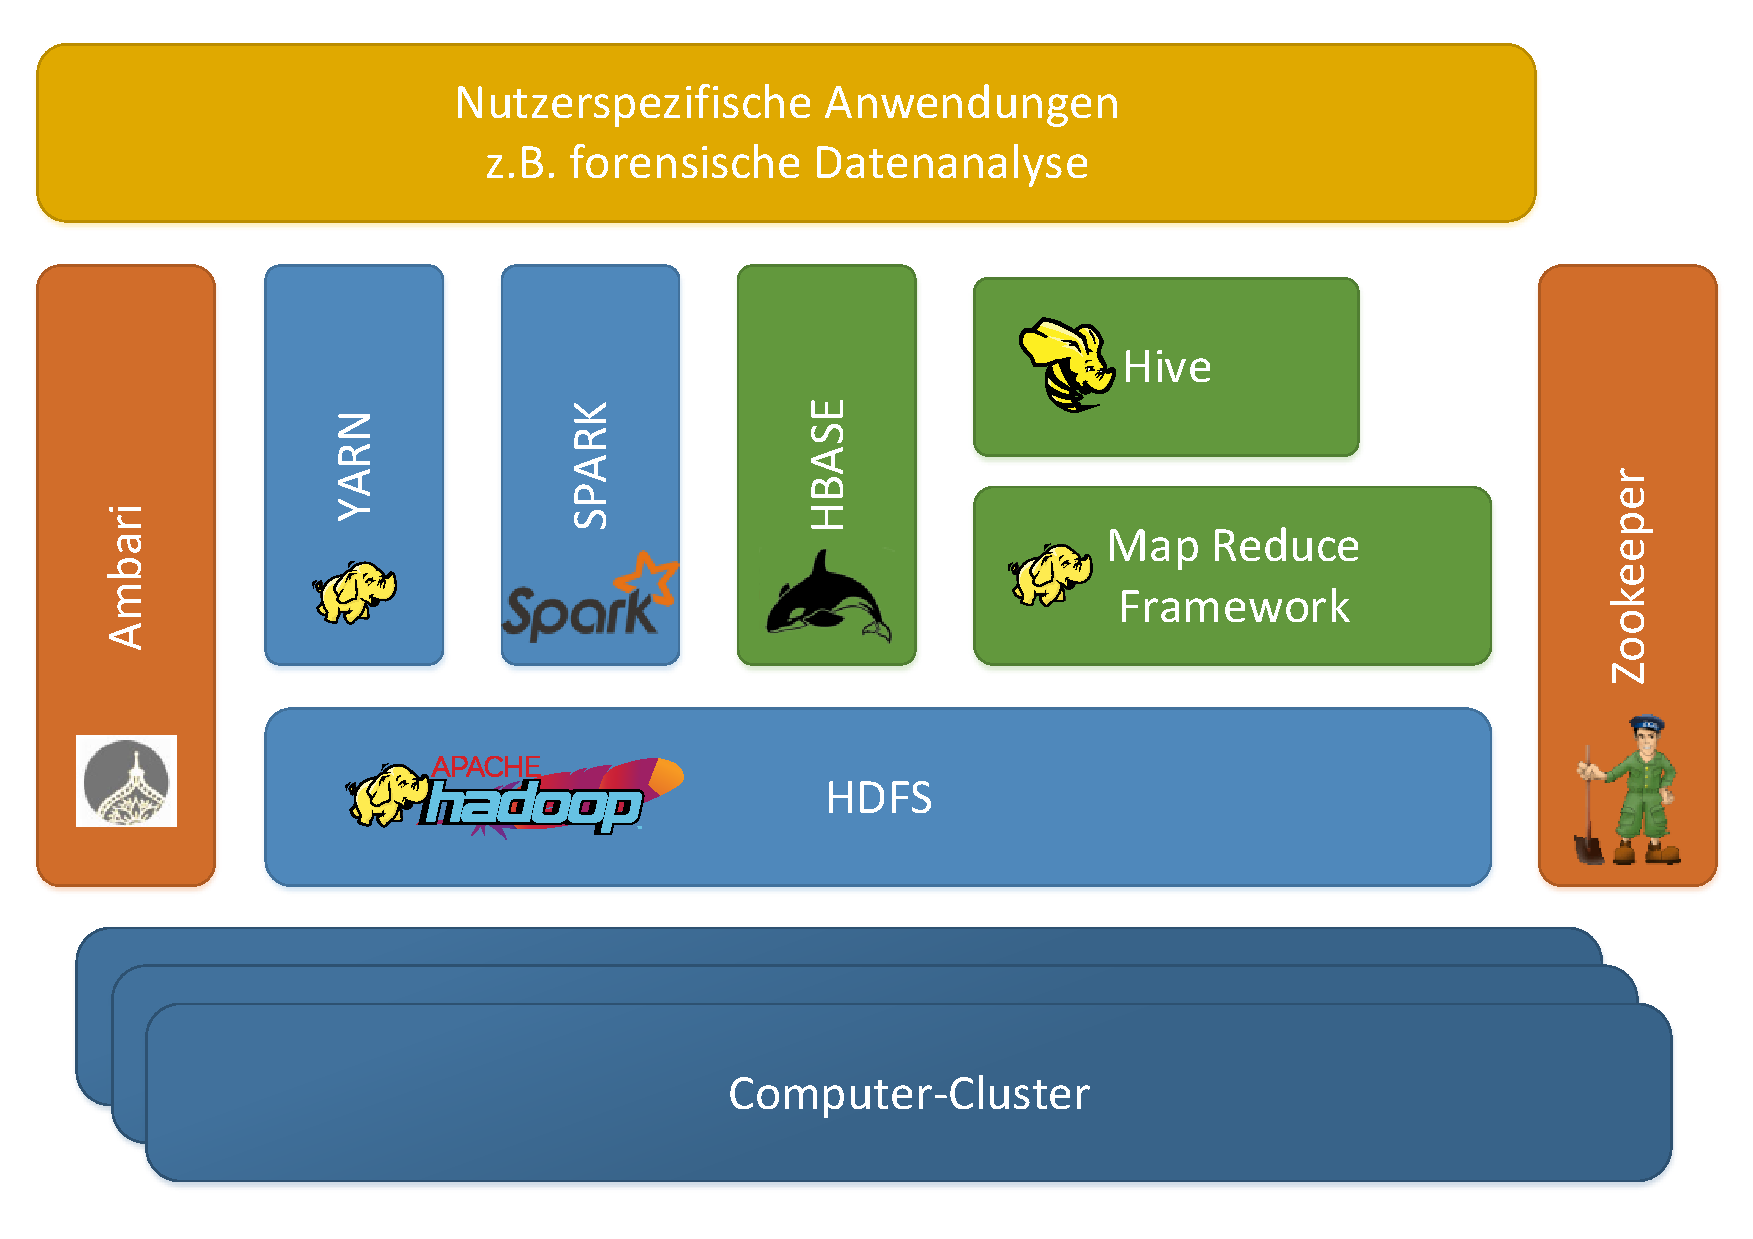
\includegraphics[width=\textwidth]{./resource/hadoop_framework_structure.pdf}
  \caption{Apache Hadoop Ökosystem (Vgl. \cite{big_data_praxis},\cite{expert_hadoop_admin}. Siehe Kapitel \ref{sec:licencing_issues})}
  \label{fig:hadoop_framework_structure}
\end{figure}

\noindent
Die Basis bildet das \textit{\gls{hdfs}}, welches die Daten redundant auf allen Knoten des Computer-Clusters speichert. Hierbei besteht das Computer-Cluster selbst aus mehreren Knoten, auf welchen vorzugsweise ein Linux-Betriebssystem, wie beispielsweise CentOS, läuft.\\
Der Ressourcenmanager \textit{\acrshort{yarn} (\acrlong{yarn})} ist für die Verteilung und Bereitstellung von verfügbarer Rechenleistung verantwortlich.\\ 
Die dritte Komponente ist das \textit{Hadoop Map-Reduce Framework}. Hadoop Map-Reduce kann zur Datenverarbeitung genutzt werden. Hierbei werden Algorithmen parallel auf den Knoten prozessiert und die Ergebnisse im Anschluss zusammengetragen. Die einzelnen Zwischenergebnisse werden alle im \gls{hdfs} abgelegt.\footnote{Sogenannte Map-Reduce Jobs bildeten in den Anfängen von Hadoop den primären Weg, Daten verteilt zu verarbeiten. Mittlerweile wurde diese Art der Datenverarbeitung in den Hintergrund verdrängt, da andere Projekte, wie beispielsweise Apache Spark, die Daten schneller verarbeiten können oder andere Ansätze zur Verarbeitung nutzen. Dies ist beispielsweise auch der Grund, weshalb Hadoop Map-Reduce in dieser Masterthesis nicht genutzt wird.} \\

\noindent
Das verteilte Dateisystem \gls{hdfs} und der Ressourcenmanager \acrshort{yarn} bilden den Kern des Hadoop-Clusters. Darauf aufbauend können andere Komponenten die Daten verarbeiten oder weitere Funktionen anbieten.
So wird beispielsweise in dieser Thesis \textit{Apache Spark\texttrademark\thinspace} bei der Prozessierung und Analyse der Daten genutzt. Der Vorteil von Apache Spark ist eine performante Datenverarbeitung, da einerseits die Daten verteilt verarbeitet werden und andererseits Zwischenergebnisse und temporäre Daten im Arbeitsspeicher der einzelnen Rechenknoten gehalten werden.\footnote{Durch das In-Memory Computing ist Apache Spark deutlich schneller als das bereits erwähnte Hadoop Map-Reduce.}\\
Des Weiteren bietet \textit{Apache Hive\texttrademark\thinspace} eine Möglichkeit, Dateien im \gls{hdfs} mithilfe einer \acrshort{sql} ähnlichen Syntax (HiveQL) abzufragen. Die Komponente nutzt wiederum das Map-Reduce Framework von Hadoop. Apache Hive ist jedoch keine reine Datenbank, sondern arbeitet auf den Dateien im \gls{hdfs}.\\
\textit{Apache HBase\textsuperscript{\textregistered}} hingegen ist eine spaltenorientierte Key-Value Datenbank. Sie wurde eigens für Apache Hadoop implementiert, 
um große Datenmengen performant zu speichern.\\

\noindent
Das Hadoop-Ökosystem als Ganzes muss auch konfiguriert und überwacht werden. Um die Verfügbarkeit einzelner Instanzen zu gewährleisten und gegebenenfalls redundante Verarbeitungswege anzubieten, wird \textit{Apache ZooKeeper\texttrademark\thinspace} genutzt. Mit ZooKeeper ist es auch möglich, Konfigurationen und Änderungen im Cluster zu verteilen. Zum eigentlichen konfigurieren und überwachen des Hadoop-Clusters wird \textit{Apache Ambari\texttrademark\thinspace} genutzt.\\

\noindent
Zusätzlich existieren dutzende weitere Projekte die auf dem Hadoop-Ökosystem aufbauen oder sich integrieren lassen. Mit \textit{Apache Accumulo\textsuperscript{\textregistered}} existiert eine weitere Key-Value Datenbank, welche eine Alternative zu HBase bietet. \textit{Apache Livy} kann zur Ausführung von Apache Spark Anwendungen, über eine \acrshort{rest}-Schnittstelle, genutzt werden.\footnote{\textit{\gls{rest}} bezeichnet ein Programmierparadigma in verteilten Systemen. Hierbei werden Ressourcen über das \gls{http} angefordert, gespeichert und verarbeitet.} \textit{Apache NiFi} hingegen ermöglicht das Aufbereiten von Daten und organisiert Datenimporte.\\
Im Rahmen dieser Thesis wird auch das bekannte Open-Source Projekt \textit{Apache Solr\texttrademark\thinspace} verwendet, um innerhalb des Hadoop-Ökosystems eine Datenindexierung für eine Volltextsuche durchzuführen.\\


\noindent
Prinzipiell sind die Komponenten auch unabhängig voneinander einsetzbar. So kann ein \gls{hdfs} ausschließlich zur Datenhaltung aufgebaut werden, ohne eine Komponente zur Datenverarbeitung verwenden zu müssen. Umgekehrt lassen sich Komponenten zur Datenverarbeitung, wie Apache Spark, auch ohne das \gls{hdfs} und YARN nutzen und können damit auch in andere Umgebungen integriert werden. Die einzelnen Komponenten entfalten, gerade durch die Kombination miteinander, ihr Potential zur performanten Datenanalyse.\\

\noindent
Es gibt einige Unternehmen, die sich darauf spezialisiert haben, das Hadoop-Ökosystem inklusive weiterer Komponenten zu einzelnen Analyseplattformen zusammenzufassen. Sie bieten dafür kostenpflichtigen Support an, wobei diese Plattformen auch kostenfrei betrieben werden können. So wird im Praxisteil der Masterthesis die \textit{\gls{hdp}} des Unternehmens \textit{Hortonworks} genutzt.


\section{Apache Hadoop HDFS}
\label{sec:theory_hdfs}
Das \acrfull{hdfs} ist ein verteiltes Dateisystem, welches die Grundlage zur Speicherung von Daten im Hadoop-Ökosystem bietet. Nachfolgende Zwecke soll es erfüllen.\\
Es soll ausfallsicher sein. In der Standardkonfiguration wird jede Datei im \gls{hdfs} dreifach auf unterschiedlichen physikalischen Knoten gespeichert. Damit kann selbst bei einem Ausfall von zwei Knoten immer noch auf die Datei zugegriffen werden. Darüber hinaus verteilt das \gls{hdfs} die Dateien automatisch und regeneriert sich selbst nach einem Knotenausfall. In großen Computer-Clustern mit mehreren hunderten Knoten ist ein Ausfall eines Knotens kein Sonderfall, sondern die Regel. Daher muss es sich selbst heilen können, um auch ohne manuelle Administration weiter verfügbar zu sein.\\
Das \gls{hdfs} (und auch Hadoop im Allgemeinen) soll horizontal skalierbar sein. Wird mehr Speicher benötigt, werden einfach weitere Knoten hinzugefügt.\\
Das \gls{hdfs} ist auf hohen Datendurchsatz und die Speicherung großer Datenmengen ausgelegt.
So können einzelne Dateien mehrere Gigabyte bis hin zu Terabyte groß sein und es können mehrere Millionen Dateien im \gls{hdfs} gespeichert werden. Die Optimierung auf einen möglichst hohen Datendurchsatz geht mit einer schlechteren Reaktionszeit, im Vergleich zu herkömmlichen Dateisystemen, einher.\\
Das Prinzip \textit{Write-once-Read-many} wird im \gls{hdfs} implementiert. Wenn Daten einmal geschrieben wurden, dann werden sie in der Regel nicht mehr geändert. Dies ermöglicht ein einfache Datenkohärenz. Der Lesedurchsatz wird gefördert, indem die Unterstützung der Datenmodifikation stark eingeschränkt wird. Ein wahlfreies Schreiben in eine existierende Datei wird beispielsweise nicht unterstützt. Änderungen an Daten, welche von Algorithmen vorgenommen werden, resultieren in neuen Datensätzen.\\

\noindent
Darüber hinaus gilt das Prinzip der Datenlokalität. Algorithmen werden dort ausgeführt, wo die Daten liegen, um das Transportieren von Daten über das Netzwerk zu vermeiden.\cite{hdfs_architecture}\\

\noindent
Der Aufbau des \gls{hdfs} bildet eine Master-Slave Architektur aus einem \textit{Name Node} und mehreren \textit{Data Nodes}. Der Name Node ist einmalig im verteilten System vorhanden und enthält alle Metainformationen zu den Dateien. Eine Datei wird in ein oder mehrere Blöcke aufgeteilt und auf mehreren Data Nodes gespeichert. Der Name Node organisiert diese Speicherung und bestimmt, wo welche Daten persistiert werden. Über den Name Node fließen aber keine Rohdaten von Dateiinhalten. Auf Dateisystemebene ist das \gls{hdfs}, wie gängige Dateisysteme, hierarchisch organisiert. Jede Datei wird über einen absoluten Pfad eindeutig bestimmt und erhält entsprechende Metadaten, wie Dateirechte und Zeitstempel.  \\

\noindent
Abbildung \ref{fig:hdfs_cluster_architecture} verdeutlicht die Struktur im \gls{hdfs}. Angenommen es soll eine Datei im \gls{hdfs} unter \path{/home/foo.txt} gespeichert werden. Dazu kann ein HDFS-Client genutzt werden, welcher Zugang zum Hadoop-Cluster hat. Der HDFS-Client speichert zuerst die Metadaten der Datei auf dem Name Node. Der Name Node kennt die Größe der Datei und entscheidet, in viele Blöcke sie unterteilt werden soll. Er ermittelt für jeden einzelnen Block, auf welchen Data Nodes dieser Block gespeichert werden soll. Diese Blockaufteilung und die Zuordnung zu den Data Nodes werden an den HDFS-Client zurückgeschickt. Dieser übermittelt die Blöcke an einen der Data Nodes. Sobald ein Data Node einen Block empfangen hat, schickt er diesen Block auch an die Knoten, welche eine Replikation des Blocks speichern sollen. Die Data Nodes stehen in Kontakt zum Name Node und senden Informationen über ihren Zustand und die momentan gespeicherten Blöcke. Der Name Node erhält dadurch auch eine Rückmeldung, falls ein Data Node ausfällt.

\begin{figure}[ht]
  \centering
  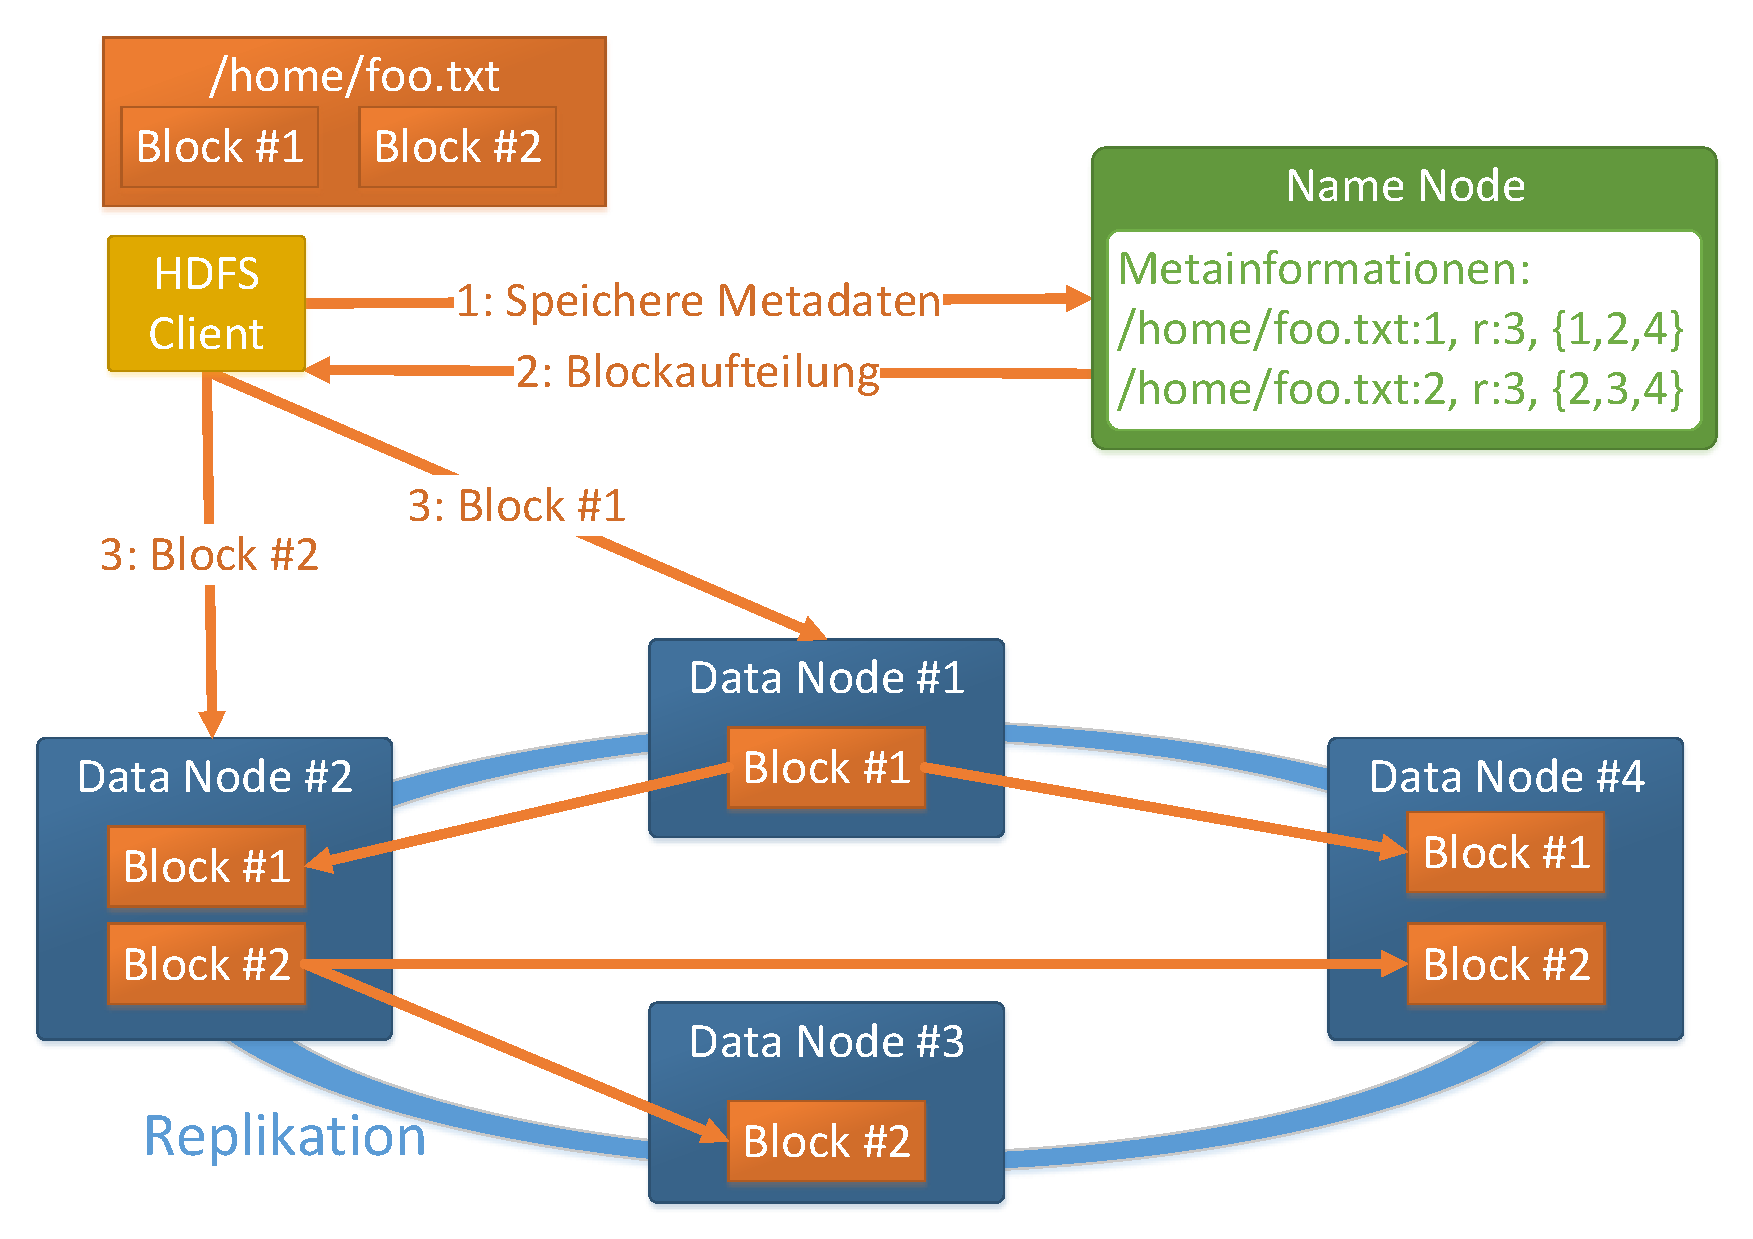
\includegraphics[width=\textwidth]{./resource/hdfs_cluster_architecture.pdf}
  \caption{HDFS - Datenspeicherung im Verbund (Vgl. \cite{hdfs_architecture},\cite{expert_hadoop_admin})}
  \label{fig:hdfs_cluster_architecture}
\end{figure}

\noindent
Ein Block ist in der Standardkonfiguration 128 MB groß. Er kann bis zu 512 MB Blockgröße konfiguriert werden. Bei der Replikation wird der gleiche Block in unterschiedlichen Data Nodes angelegt.\\
Es ist nicht erlaubt, den gleichen Block mehrmals im gleichen Data Node zu replizieren. Dies wäre ohnehin sinnfrei, da die Replikation gerade vor einem Datenverlust, bei Ausfällen von einzelnen Knoten, schützen soll. Wichtig hierbei ist auch, dass im Produktivsystem auf jedem physikalischen Knoten nur ein Data Node oder ein Name Node läuft. Denn würden beispielsweise mehrere Data Nodes auf dem gleichen physikalischen Knoten laufen, so wäre bei einem Ausfall nicht mehr garantiert, dass die Dateiinhalte auch noch auf mindestens zwei anderen verfügbaren Knoten gespeichert sind.
Denn der Replikationsmechanismus im \gls{hdfs} kann nicht erkennen, ob jeder Knoten physikalisch unabhängig arbeitet. Allerdings hat Hadoop eine sogenannte \textit{Rack-Awareness}. So ist es möglich, zu bestimmen, welche physikalischen Knoten in einem gemeinsamen Rack gruppiert sind. Abhängig davon, versucht das \gls{hdfs} die Daten teilweise im selben Rack redundant zu speichern aber auch einige Replikationen außerhalb des Racks anzulegen. So kann auch der Ausfall eines Racks im Notfall kompensiert werden.\\
In einzelnen Testumgebungen ist es aber durchaus möglich, einen Name Node und einen Data Node oder mehrere Data Nodes gemeinsam auf einem physikalischen Knoten zu installieren. Allerdings greifen dann die eben beschriebenen Mechanismen zur Datensicherheit gegenüber Hardwareausfällen nicht mehr.\\

\noindent
Wie in Abbildung \ref{fig:hdfs_cluster_architecture} ersichtlich, ist der Name Node die Schlüsselstelle im HDFS-Cluster. Zusätzlich existiert ein sogenannter \textit{Secondary Name Node}, der den (First) Name Node beim Speichern von Daten in gewisser Hinsicht unterstützt. Der Name Node hält die Metainformationen des \gls{hdfs} im Arbeitsspeicher. Zusätzlich existieren zwei Dateien, das sogenannte \textit{FsImage} und ein \textit{EditLog}, welche persistent auf der Festplatte gespeichert sind. Das FsImage beschreibt einen Zustand der Dateisystemmetainformationen zu einem gewissen Zeitpunkt (Checkpoint). Im EditLog befinden sich alle Änderungen seit dem letzten Checkpoint bis zum aktuellen Zeitpunkt.\\
Der Secondary Name Node erstellt aus dem FsImage und dem EditLog regelmäßig neue Checkpoints, welche wiederum als neue FsImages gespeichert werden.
Dieser Mechanismus wurde implementiert, um bei einem Neustart des Name Nodes die Startzeit zu optimieren. Dadurch kann die Verfügbarkeit des gesamten \gls{hdfs}  verbessert werden. Der \textit{Secondary Name Node} unterstützt also den (First) Name Node, er kann ihn aber nicht ersetzen. Bei einem Ausfall wäre das \gls{hdfs} nicht mehr einsatzbereit. Um dieses Problem zu umgehen, kann ein sogenannter \textit{Standby Name Node} konfiguriert werden. Dieser kann einspringen, sobald der erste Name Node ausgefallen ist. Allerdings muss er extra konfiguriert werden.\cite[S. 40 ff.]{expert_hadoop_admin}\\

\noindent
Das \gls{hdfs} kann über mehrere Wege genutzt werden. Es gibt eine Kommandozeilenschnittstelle, die sogenannte \textit{FS Shell}. Mit der FS Shell können simple Dateioperationen durchgeführt werden. Die Befehlssyntax ähnelt hierbei stark der Befehlssyntax von UNIX/Linux-Betriebssystemen. Es ist auch möglich, über eine Java oder C++-Schnittstelle auf die Daten zuzugreifen. Das Dateisystem kann über eine \gls{rest}-Schnittstelle via \gls{http}(S) genutzt werden. Auch das Mounten als \textit{\gls{nfs}} ist möglich. Das HDFS bietet auch eine Web-Oberfläche an, die es erlaubt, Daten auf einfache Weise hoch- und herunterzuladen.

\section{Apache Hadoop YARN}
\label{sec:theory_yarn}
\acrshort{yarn} (\acrlong{yarn}) ist eine Ressourcenverwaltung, welche die verfügbaren Ressourcen innerhalb des Hadoop Clusters organisiert und die Ausführungsreihenfolge von Jobs plant und überwacht. Es gibt einen separaten \textit{Resource Manager}, welcher nur die Ressourcen verwaltet. Auf jedem Knoten, der auch Datenverarbeitungen durchführt, ist ein \textit{Node Manager} installiert. Zuletzt gibt es noch einen \textit{Application Manager} für jeden einzelnen Job, der ausgeführt werden soll. Der Application Manager kontrolliert die Ausführung des Jobs.
Abbildung \ref{fig:yarn_cluster_architecture} zeigt die Komponenten von YARN im Cluster.\\

\begin{figure}[ht]
  \centering
  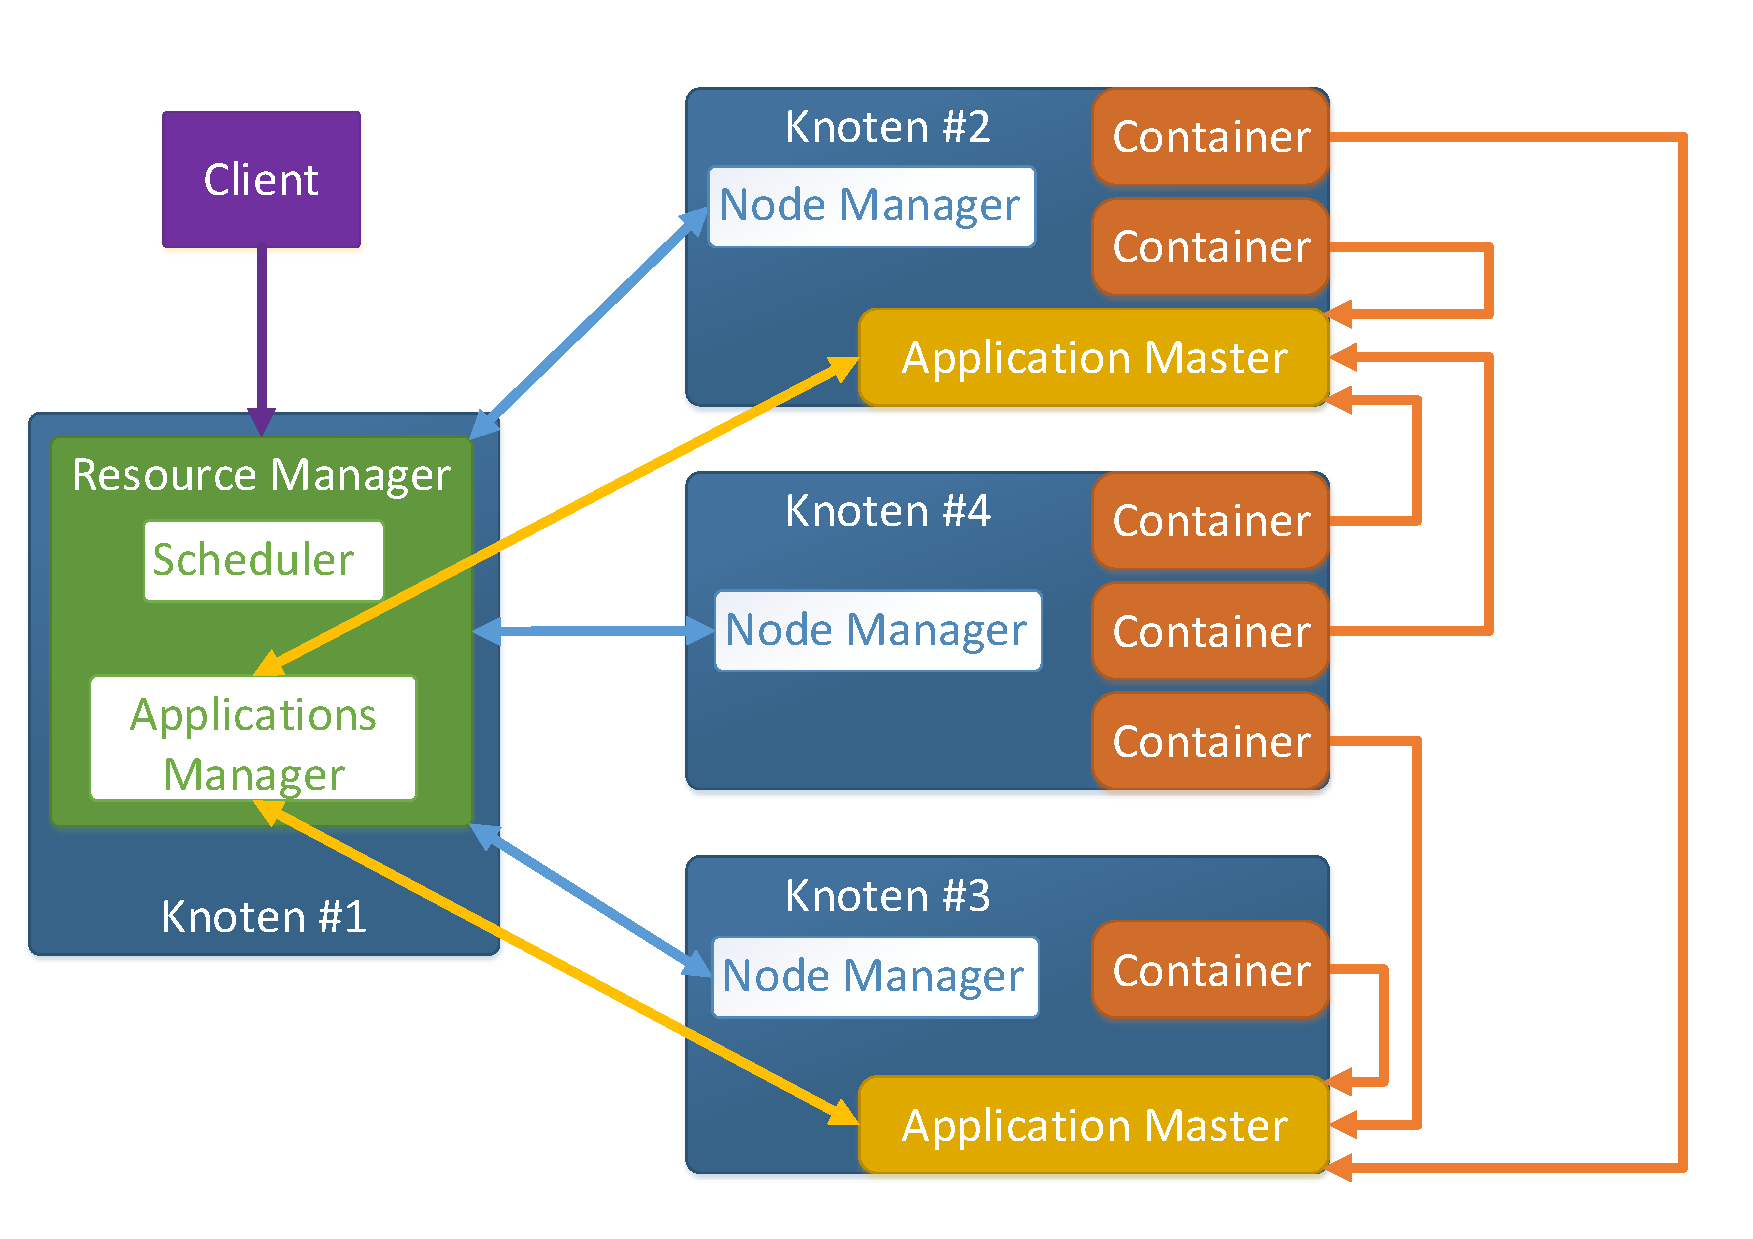
\includegraphics[width=\textwidth]{./resource/yarn_cluster_architecture.pdf}
  \caption{Ressourcenverteilung mit YARN (Vgl. \cite{yarn_architecture},\cite{expert_hadoop_admin})}
  \label{fig:yarn_cluster_architecture}
\end{figure}

\noindent
Ein Job oder eine Anwendung besteht aus mehreren Tasks. Diese Tasks können parallel in mehreren Containern ausgeführt werden. Ein Container ist eine abstrakte parallele Verarbeitungseinheit, welcher vordefinierte \acrshort{cpu}- und Speicher-Ressourcen enthält. Es können mehrere dieser Container auf einem Knoten innerhalb des Clusters ausgeführt werden. Beispielsweise werden bei einem Knoten mit einer Quad-Core CPU und Hyperthreading (mit insgesamt 8 ausführbaren Threads) bis zu 8 Container erstellt. Bei 32 GB verfügbarem Arbeitsspeicher werden jedem Container 4 GB zugeteilt.\footnote{In der Praxis ist es meistens weniger, da entsprechende Ressourcen für das darunter liegende Betriebssystem und die Hadoop-Komponenten reserviert werden.}\\
Es ist nur möglich, die Anzahl der CPU-Cores (Ausführbare CPU-Threads) und die Größe des nutzbaren Arbeitsspeichers als Konfigurationsparameter festzulegen.\cite[S. 48-57]{expert_hadoop_admin}\\ In den meisten Fällen sind diese beiden Parameter ausschlaggebend, um die Parallelität und den Ressourcenverbrauch des Systems zu steuern.

\noindent
Wenn nun eine Anwendung über YARN im Cluster ausgeführt werden soll, dann sendet ein Client eine Anfrage an den Resource Manager. 
Für jeden auszuführenden Job erstellt der Resource Manager den ersten Container. In diesem Container wird dann der Application Master gestartet, welcher sich im weiteren Verlauf um die Ausführung des Jobs kümmert. Der Resource Manager kennt die Anwendung nicht, noch weiß er wie diese ausgeführt wird. 
Er ist nur dafür zuständig, Ressourcen zu verteilen.\\ 
Der Application Master hingegen ist sehr spezifisch. Wird zum Beispiel eine Apache Spark Anwendung mit YARN ausgeführt, so ist der Application Master der sogenannte \textit{Spark App Master}. Nachdem der Application Master im ersten erzeugten Container gestartet wurde, kann dieser wiederum neue Ressourcen beim Resource Manager anfordern. 
An dieser Stelle zeigt sich der Vorteil von YARN in Kombination mit dem \gls{hdfs}. Denn bei der Anforderung von Ressourcen gibt der Application Master an, wie viele Container (inklusive Arbeitsspeicher und CPU) er benötigt. Zusätzlich übermittelt er die Dateiblöcke, welche er aus dem \gls{hdfs} braucht und auf welchen Knoten er wie viele Container starten will.\\ 
In Abbildung \ref{fig:yarn_cluster_architecture} fordert der Application Master des Knoten \#2 einen Container auf dem gleichen Knoten an. Zusätzlich möchte er zwei Container auf dem Knoten \#4 erstellen. Der Application Master weiß, dass dort die benötigten Datenblöcke im \gls{hdfs} gespeichert sind. Hierbei ist es wichtig zu verstehen, dass die Knoten aus Abbildung \ref{fig:yarn_cluster_architecture} den Data Nodes des HDFS aus Abbildung \ref{fig:hdfs_cluster_architecture} entsprechen.\footnote{Wobei ein physikalischer Knoten, auf welchem ein Data Node läuft, nicht zwingend auch für die Datenverarbeitung mit YARN verwendet werden muss. Beziehend auf das Paradigma der Datenlokalität ist es aber üblich, dass ein Knoten, welcher Daten persistiert, auch Daten verarbeitet.}\cite[S. 48-57]{expert_hadoop_admin}\\
Der Application Master erhält die Zustimmung vom Resoure Manager, nachdem der Scheduler die geforderten Ressourcen entsprechend eingeteilt hat. Zusätzlich befiehlt der Resource Manager den Node Managern auf den jeweiligen Knoten, entsprechende Container zu erstellen.\\
Die einzelnen Node Manager stehen in Kontakt zum Resource Manager und senden ihm den aktuellen Status des Knotens und dessen Auslastung. \\
%TODO Nachfolgende Aussage muss nochmals geprüft werden.
Nach der Ausführung der einzelnen Tasks in den Containern und dem Abschluss des Jobs, schickt der Application Master über den Applications Manager die Ergebnisse zurück zum Client.\footnote{Hierbei werden die fachlichen Ergebnisse meistens als Datei im \gls{hdfs} gespeichert.} Danach meldet er sich beim Resource Manager. Zum Schluss gibt der Resource Manager die allokierten Ressourcen wieder frei.\\


\noindent
Ähnlich wie beim Prozessscheduling in einem Betriebssystem, gibt es auch für YARN unterschiedliche Algorithmen, die festlegen, in welcher Reihenfolge und Zeitdauer die einzelnen Jobs ausgeführt werden. Bekannte Scheduler sind der \textit{Fair Scheduler} und der \textit{Capacity Scheduler}. Abhängig von der genutzten Plattform/Distribution einzelner Hersteller, ist für YARN ein anderer Scheduler konfiguriert.\\
Der Capacity Scheduler ist als Standard konfiguriert, da dieser versucht alle Knoten möglichst effizient auszusteuern, um den höchstmöglichen Datendurchsatz zu erreichen. Der Fair-Scheduler prüft hingegen, dass jedem Job die gleichen Ressourcen zugeteilt werden, um möglichst alle Jobs parallel bedienen zu können.\\

\noindent
In großen Clustern wird die Prozessierung in mehrere Sub-Cluster, mit eigenen Resource Managern, aufgeteilt. Diese Struktur wird in der Literatur als \textit{Federaded YARN} beschrieben und soll die Skalierbarkeit von YARN in großen Clustern ermöglichen.

\section{Apache Spark}
\label{sec:theory_spark}

\textit{Apache Spark\texttrademark\thinspace} ist ein Framework zur verteilten Verarbeitung von großen Datenmengen. Mit Apache Spark können verschiedene Algorithmen und Verarbeitungsschritte über eine einheitliche Programmierschnittstelle auf gespeicherte Daten  angewendet werden. Spark kümmert sich dabei um die Verteilung, Ausführung und Überwachung der datenverarbeitenden Applikationen.\cite[S. 2]{learning_spark}\\
Apache Spark ist mittlerweile schon fast der Standard, wenn es im Hadoop-Umfeld um die Datenverarbeitung geht. Es löst damit auch das ursprünglich verwendete Map Reduce Framework von Hadoop ab, denn Spark bietet einen enormen Geschwindigkeitsvorteil gegenüber von Hadoop Map Reduce. Dies lässt sich auf eine intelligente Ausführung einzelner Verarbeitungsschritte und diverse Optimierungen zurückführen.\cite[S. 148-153]{expert_hadoop_admin}\\

\noindent
Spark ermöglicht vielseitige Einsatzzwecke. So wird die klassische Datenverarbeitung von statischen Datenmengen\footnote{In diesem Kontext ist die simple Ausführung einer Anwendung auf eine bereits existierende Datenmenge gemeint, welche am Ende ein definiertes Ergebnis liefert.} unterstützt, aber auch die Verarbeitung von dynamischen Datenmengen (Streaming-Data).\footnote{Bei der Datenverarbeitung von Streaming-Data wächst die zu verarbeitende Datenmenge dynamisch an, während die ausgeführte Anwendung die neu hinzugekommenen Daten verarbeitet. Ein Beispiel hierzu ist das Filtern von Tweets auf Twitter, wobei auch neu hinzukommende Tweets bearbeitet werden und nicht nur die Tweets, welche beim Startzeitpunkt der Anwendung bereits existieren.} Auch die Prozessierung von Graphen-Strukturen und das maschinelle Lernen werden unterstützt.\cite[S. 152]{expert_hadoop_admin}\\

\noindent
Darüber hinaus steht es dem Anwender frei, ob er seine Applikationen in Scala, Python oder Java schreibt. Bei den Skriptsprachen Scala und Python gibt es eine Spark-Shell zur interaktiven Datenverarbeitung und Analyse. Diese Vielseitigkeit macht sich auch in unzähligen Projekten und Programm-Bibliotheken bemerkbar, welche rund um Apache Spark entwickelt werden.
Es existieren sogenannte \textit{Spark-Connectoren}, welche die Verbindung zu anderen Komponenten herstellen. Damit können diverse Datenspeicher als Datenquelle verwendet werden. Beispielsweise können Daten aus dem \gls{hdfs} geladen werden. Oder die Daten werden aus anderen Datenspeichern, wie HBase, Cassandra, Neo4j oder Elasticsearch gelesen.\\

\noindent
Abbildung \ref{fig:spark_cluster_architecture} zeigt die Ausführung einer Spark-Applikation mit YARN. Es wird der physikalische Kontext innerhalb eines Hadoop-Clusters dargestellt. Dieser Aufbau beschreibt im Rahmen der Thesis den primären Anwendungsfall zur Datenverarbeitung.\\ 
Apache Spark kann auch vollständig unabhängig von dem Hadoop-Framework, in einem eigenen Spark-Cluster, ausgeführt werden und bietet dafür einen eigenen Ressourcenmanager.\\
Allerdings wird innerhalb des Hadoop-Umfelds die Spark-Ausführung mit dem bereits erwähnten Ressourcenmanager YARN durchgeführt (siehe Kapitel \ref{sec:theory_yarn}). 
Dies hat den Vorteil, dass YARN die Ressourcen auf den einzelnen Knoten besser verwalten kann. Wenn der Spark-Ressourcenmanager parallel zu YARN auf den gleichen Knoten genutzt wird, so kann dies zu Ressourcen-Engpässen führen. 
Denn die Ressourcenmanager würden nicht miteinander kommunizieren und die Last der ausgeführten Anwendungen im Cluster könnte nicht gleichmäßig verteilt werden. Aus diesem Grund ist es ratsam, YARN auch die Ausführung von Spark-Anwendungen im Cluster zu überlassen.\\

\begin{figure}[ht]
  \centering
  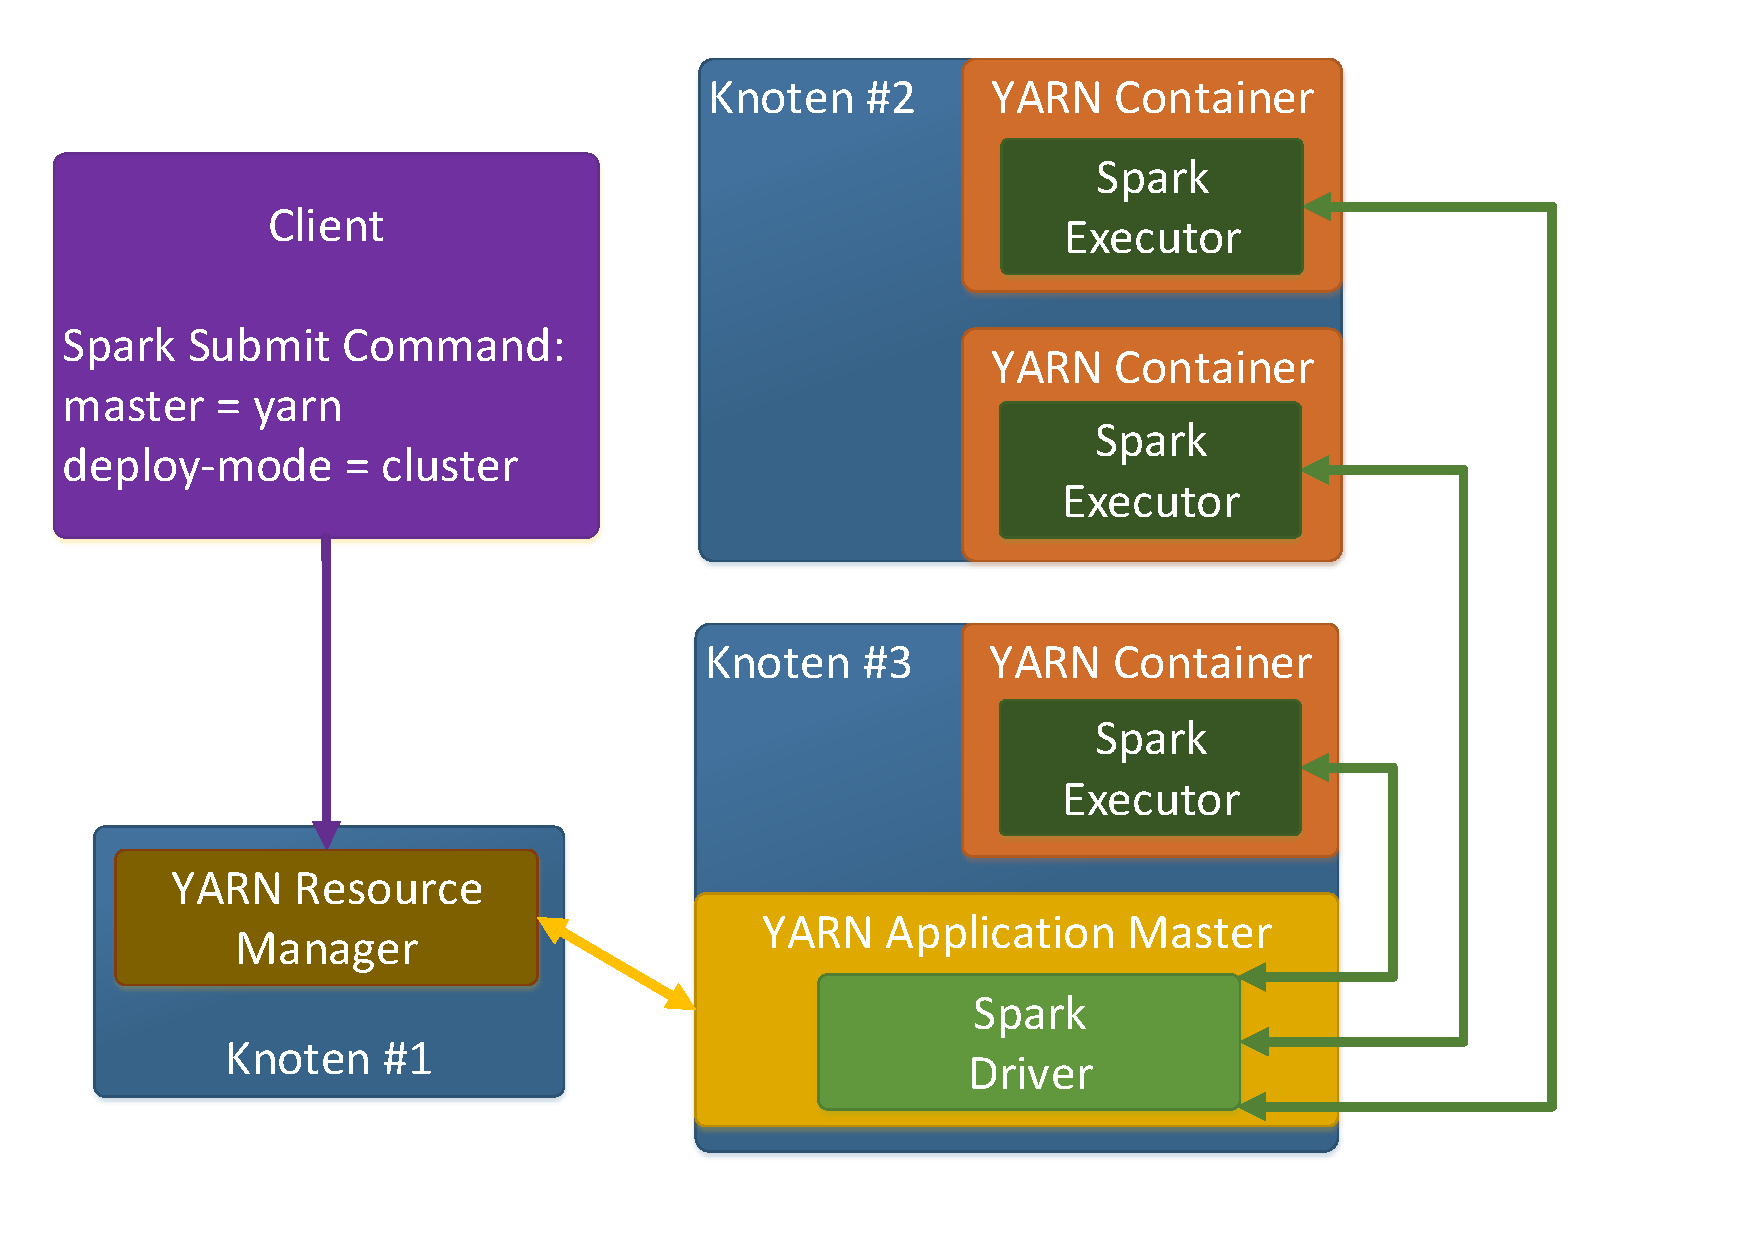
\includegraphics[width=\textwidth]{./resource/spark_cluster_architecture.pdf}
  \caption{Spark Datenverarbeitung im Cluster}
  \label{fig:spark_cluster_architecture}
\end{figure}

\noindent
Wie in Abbildung \ref{fig:spark_cluster_architecture} ersichtlich, wird die Ausführung einer Spark-Anwendung über den YARN-Ressourcenmanager gestartet. Es gibt hierbei unterschiedliche Varianten, wie eine Spark-Anwendung ausgeführt werden kann. 
Im konkreten Fall wird das \textit{Spark-Submit}-Kommando genutzt. Letztlich handelt es sich dabei um einen Konsolenbefehl, welcher die eigentliche Anwendung\footnote{Bei einer Spark-Anwendung, welche in Java geschrieben wurde, besteht die Applikation aus einem herkömmlichen \textit{Java Archiv} im \textit{\gls{jar}}-Dateiformat.} entgegen nimmt und über diverse Parameter konfiguriert werden kann. 
Damit YARN die Ressourcen der Applikation verwaltet, müssen die Parameter \textit{Master} und \textit{Deploy Mode} entsprechend angepasst werden. Wie in Abbildung \ref{fig:yarn_cluster_architecture} (siehe Kapitel \ref{sec:theory_yarn}) bereits beschrieben, wird bei YARN ein Application Master erstellt, welcher wiederum diverse Ausführungscontainer auf den einzelnen Knoten anfordert und diese überwacht. Bei der Ausführung einer Spark-Anwendung werden diese Komponenten wiederverwendet und kapseln letztlich die fachlichen Komponenten von Spark.\\
So gibt es bei Spark einen sogenannten \textit{Driver}, welcher im YARN Application Master läuft und die sogenannten \textit{Executor} aussteuert. Diese werden in einzelnen YARN Containern auf den Knoten ausgeführt. Ein Spark Executor entspricht, aus Sicht des Betriebssystems eines Knotens, der Ausführung einer \gls{jvm} in einem eigenständigen Prozess. Aufgrund der Kapselung durch YARN, können die einzelnen \gls{jvm}-Prozesse überwacht und zur Not auch beendet werden, falls sie zu viel Ressourcen auf den Knoten anfordern.\\

\noindent
Spark und YARN müssen entsprechend konfiguriert sein, damit die Anwendungen korrekt im Cluster skaliert werden. Analog zur YARN wird bei Spark die Anzahl der genutzten CPU-Cores und die Größe des genutzten Arbeitsspeichers konfiguriert.\\
Wenn YARN einzelne Application-Container stoppt, weil sie zu viel Arbeitsspeicher benötigen, dann deutet dies meistens auf eine falsche Konfiguration oder falsche Programmierung der Spark-Anwendungen hin. Um das Problem zu lösen, wird oftmals der nutzbare Arbeitsspeicher pro Executor höher konfiguriert. Dies ist in den meisten Fällen jedoch der falsche Ansatz, da hierdurch kritische Probleme in der Programmlogik der Anwendung nur kaschiert werden.\\ 
Daher ist es sinnvoll, bei der Anwendungsentwicklung relativ kleine Cluster mit geringen Ressourcen zu nutzen, denn auch dort müssen die Anwendungen fehlerfrei ausführbar sein. Lediglich die Ausführungsgeschwindigkeit sollte sich in kleinen Clustern verlangsamen. Aus diesem Grund werden im Rahmen der Thesis die Spark-Anwendungen auch auf einem einzelnen Knoten getestet, um Programmfehler besser und früher erkennen zu können. Einzelheiten zu den Programmierparadigmen und den grundlegenden Datenstrukturen, sind in Kapitel \ref{ch:data_processing} beschrieben.


\section{Apache HBase}
\label{sec:theory_hbase}
\textit{Apache HBase\textsuperscript{\textregistered}} ist eine spaltenorientierte \textit{\acrshort{nosql}}-Datenbank. Sie entstand auf den Grundlagen der \textit{BigTable}-Datenbank von Google und wurde für das Speichern von Daten im Hadoop-Umfeld entwickelt.\footnote{Der Name \textit{HBase} basiert auf der Kombination von \textit{Hadoop} und \textit{Database}.}\\
Der Begriff \textit{NoSQL}-Datenbank steht hierbei für \textit{Not only SQL} und beschreibt letztlich Datenbanken, welche Daten vorwiegend nicht in herkömmlichen relationalen Datenbankschemata speichern. Größtenteils sind diese Datenbanken schemafrei und können horizontal skaliert werden. Diese Bedingungen sind optimal zur Speicherung großer unstrukturierter Datenmengen.\\
Anhand des sogenannten \textit{\acrshort{cap}-Theorems} können diese Datenbanken kategorisiert werden.
Das CAP-Theorem besteht aus den Eigenschaften Konsistenz, Verfügbarkeit und Partitionstoleranz und besagt, dass maximal zwei dieser drei Eigenschaften von einer Datenbank garantiert werden können. Konsistenz beschreibt hier die Garantie, dass alle Knoten im verteilten System den gleichen Datenstand haben. Die Verfügbarkeit bezieht sich auf die dauerhafte Erreichbarkeit der Daten. Wohingegen die Partitionstoleranz die Funktionsfähigkeit bei einem Ausfall einzelner Knoten im Datenbank-Verbundsystem garantiert.
Apache HBase garantiert die Eigenschaften der Partitionstoleranz und der Konsistenz. Dies führt dazu, dass die Verfügbarkeit der Daten weniger stark ausgeprägt ist.
\cite[S. 189 ff.]{big_data_praxis}\\
% Vielleicht wäre auch hier eine Überlegung die Datenbank Cassandra zu nutzen, welche die Verfügbarkeit und Partitionstoleranz garantiert. An sich genommen ist die Konsistenz der Ergebnisse in der Forensik schon wichtig, allerdings sind nach der ersten Datenalyse eigentlich keine Änderungen auf den existierenden Datensätzen zu erwarten. Vielleicht wäre dann die Konsistenzgarantie ein Stück weit überflüssig und Cassandra könnte bessere Performanz bieten?

\noindent
Während bei klassischen relationalen Datenbanken die Daten zeilenweise in Tabellen strukturiert werden, wird in spaltenorientierten Datenbanken hingegen eine andere Struktur genutzt. Die Daten werden in einzelnen Spalten gruppiert und in sogenannten \textit{Column Families} abgespeichert. Der Vorteil dieser Speicherart hängt stark von deren fachlichen Nutzung ab. Wenn alle Daten einer Spalte abgefragt werden, dann können diese Daten effizient gelesen werden, da sie zusammen persistiert wurden.\\ 
Apache HBase basiert auf dieser Spaltenorientierung. Die Datenbank wird im Rahmen der Thesis für das Speichern beliebiger Dateiinhalte und Dateimetadaten verwendet. Ein vereinfachtes Beispiel einer möglichen Datenstruktur wird in Abbildung \ref{fig:hbase_schema_example} dargestellt.\\

\begin{figure}[ht]
  \centering
  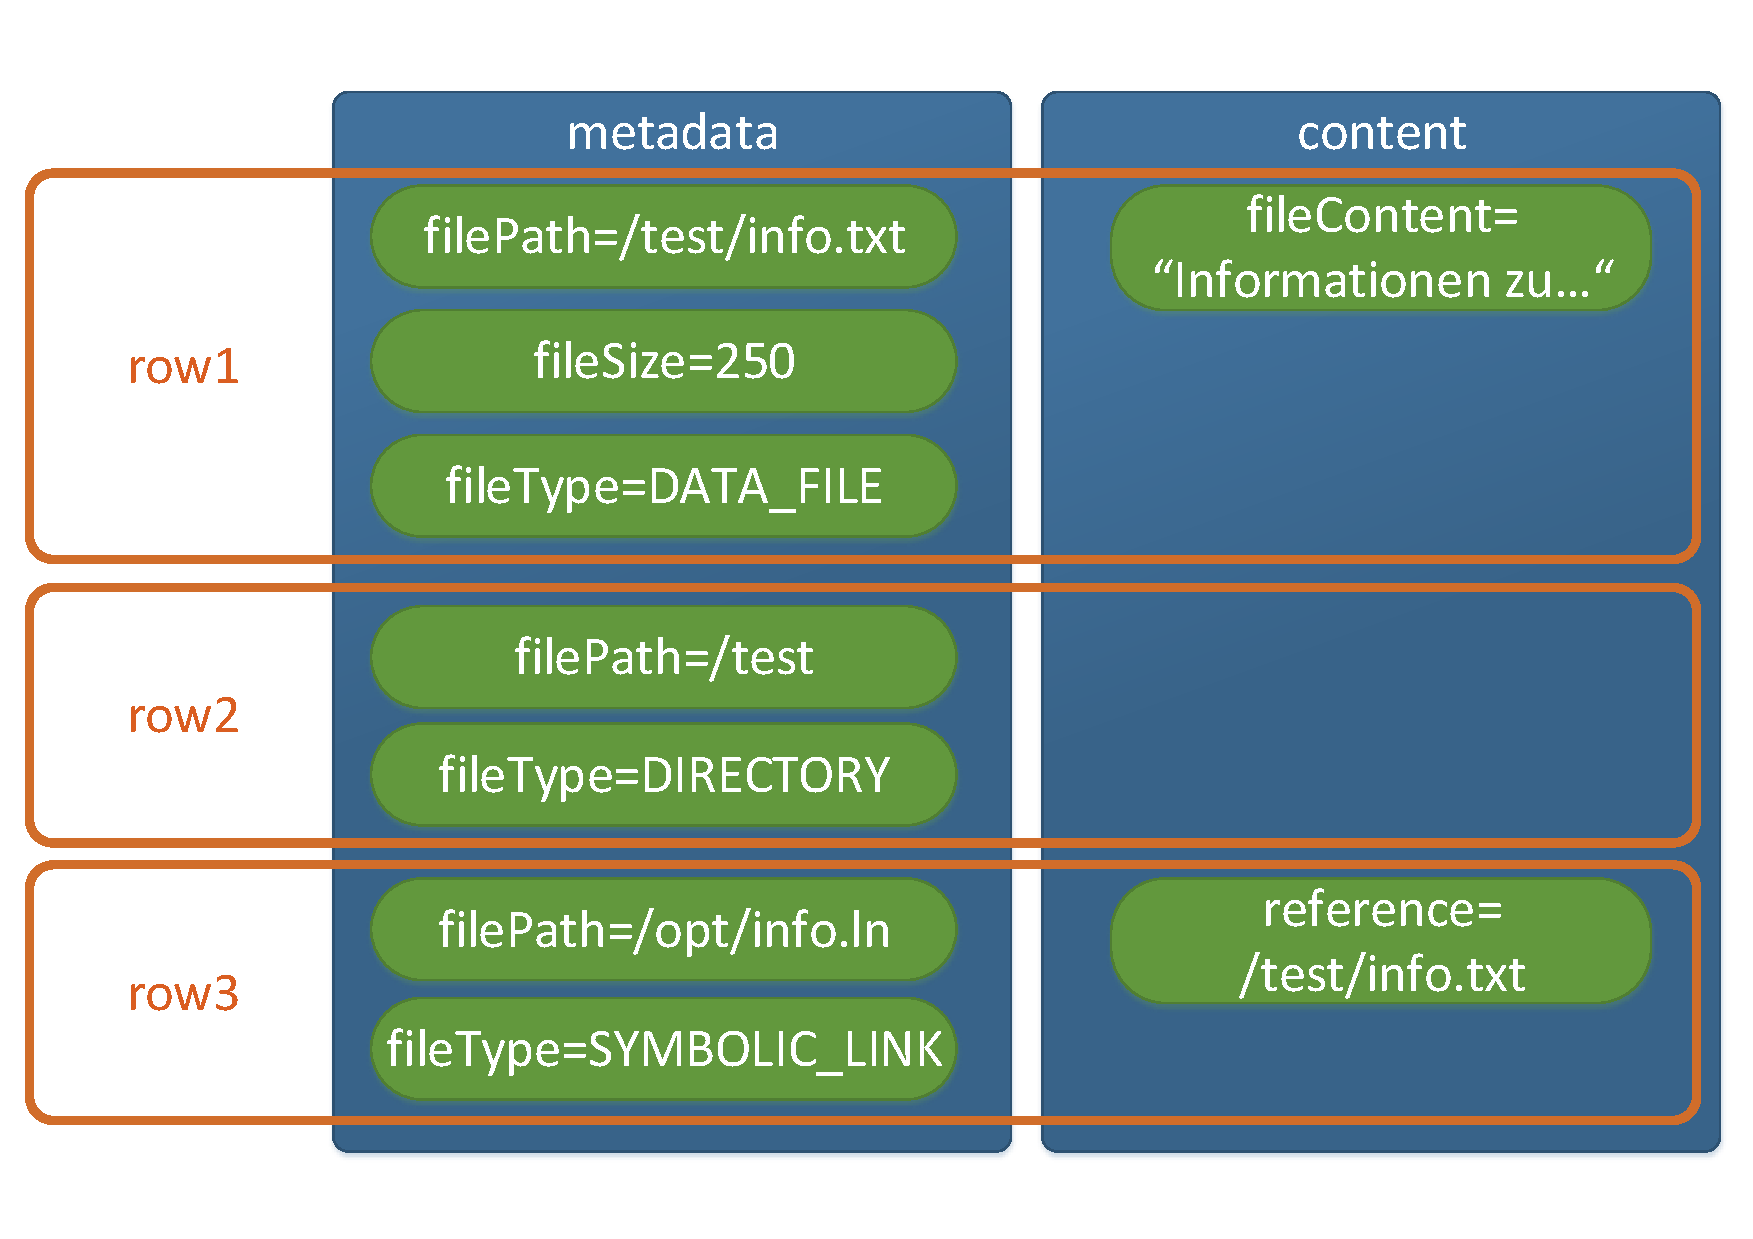
\includegraphics[width=0.8\textwidth]{./resource/hbase_data_schema_example.pdf}
  \caption{Schema-Beispiel einer HBase Tabelle (Vgl. \cite{big_data_praxis})}
  \label{fig:hbase_schema_example}
\end{figure}

\noindent
Anhand der Abbildung werden einige Eigenschaften von HBase sichtbar. So existieren zwei \textit{Column Families} mit den Namen \textit{metadata} und \textit{content}. Die Column Family \textit{metadata} enthält wiederum die Spalten \textit{filePath}, \textit{fileSize}und \textit{fileType}. Alle Werte werden als Binär-Inhalt gespeichert. Eine Zeile hat einen eindeutigen Spaltenschlüssel, wie zum Beispiel \textit{row1}. 
Über diesen Schlüssel können die spezifischen Inhalte der einzelnen Spalten für eine bestimmte Zeile erfragt werden. Interessant hierbei ist, dass die Spaltenwerte optional sind und nicht für jede Zeile existieren müssen. So hat eine Datendatei einen konkreten Inhalt, welcher in der Spalte \textit{fileContent} der Spaltenfamilie \textit{content} gespeichert wird. Wohingegen ein Verzeichnis keinen Dateiinhalt halt. 
Daher ist in der zweiten Zeile auch kein Inhalt in der Spalte \textit{fileContent} abgelegt. In der dritten Zeile wird ein symbolischer Link gespeichert. Dieser hat auch keinen Inhalt in der Spalte \textit{fileContent}. Dafür wird aber die Referenz auf die Originaldatei in einer weiteren Spalte gespeichert. Aufgrund der Gruppierung und Speicherung in Column Families, benötigen leere Spaltenwerte auch keinen Speicherplatz.\\ 

\noindent
Eine einzelne Zelle beschreibt letztlich den Wert einer Spalte für eine konkrete Zeile. Hierbei wird zu jeder Zelle auch ein Zeitstempel gespeichert. Durch die Zeitstempel können ältere Werte einer Zelle ausgelesen werden. 
So wird bei einer Modifikation einer konkreten Zelle der Wert zusammen mit einem neuen Zeitstempel geschrieben.\\
Die einzelnen Spalten innerhalb einer Spaltenfamilie müssen nicht bei der Erstellung einer Tabelle bekannt sein. Lediglich die Spaltenfamilien müssen initial angegeben werden und können später auch nicht mehr geändert werden. Dadurch ist eine nachträgliche Erweiterung der Tabelle, um zusätzliche Spalten, problemlos möglich.\cite[S. 577]{hadoop_definitive_guide}\\

\noindent
Die Skalierbarkeit und die Partitionstoleranz wurden bei der Entwicklung von HBase berücksichtigt. Es baut auf dem Hadoop \gls{hdfs} auf und speichert darin die Daten. Analog zu \gls{hdfs}, YARN und Spark existiert eine Master-Slave Architektur über alle Knoten hinweg. Abbildung \ref{fig:hbase_cluster_architecture} zeigt die physikalische Aufteilung.\\

\begin{figure}[ht]
  \centering
  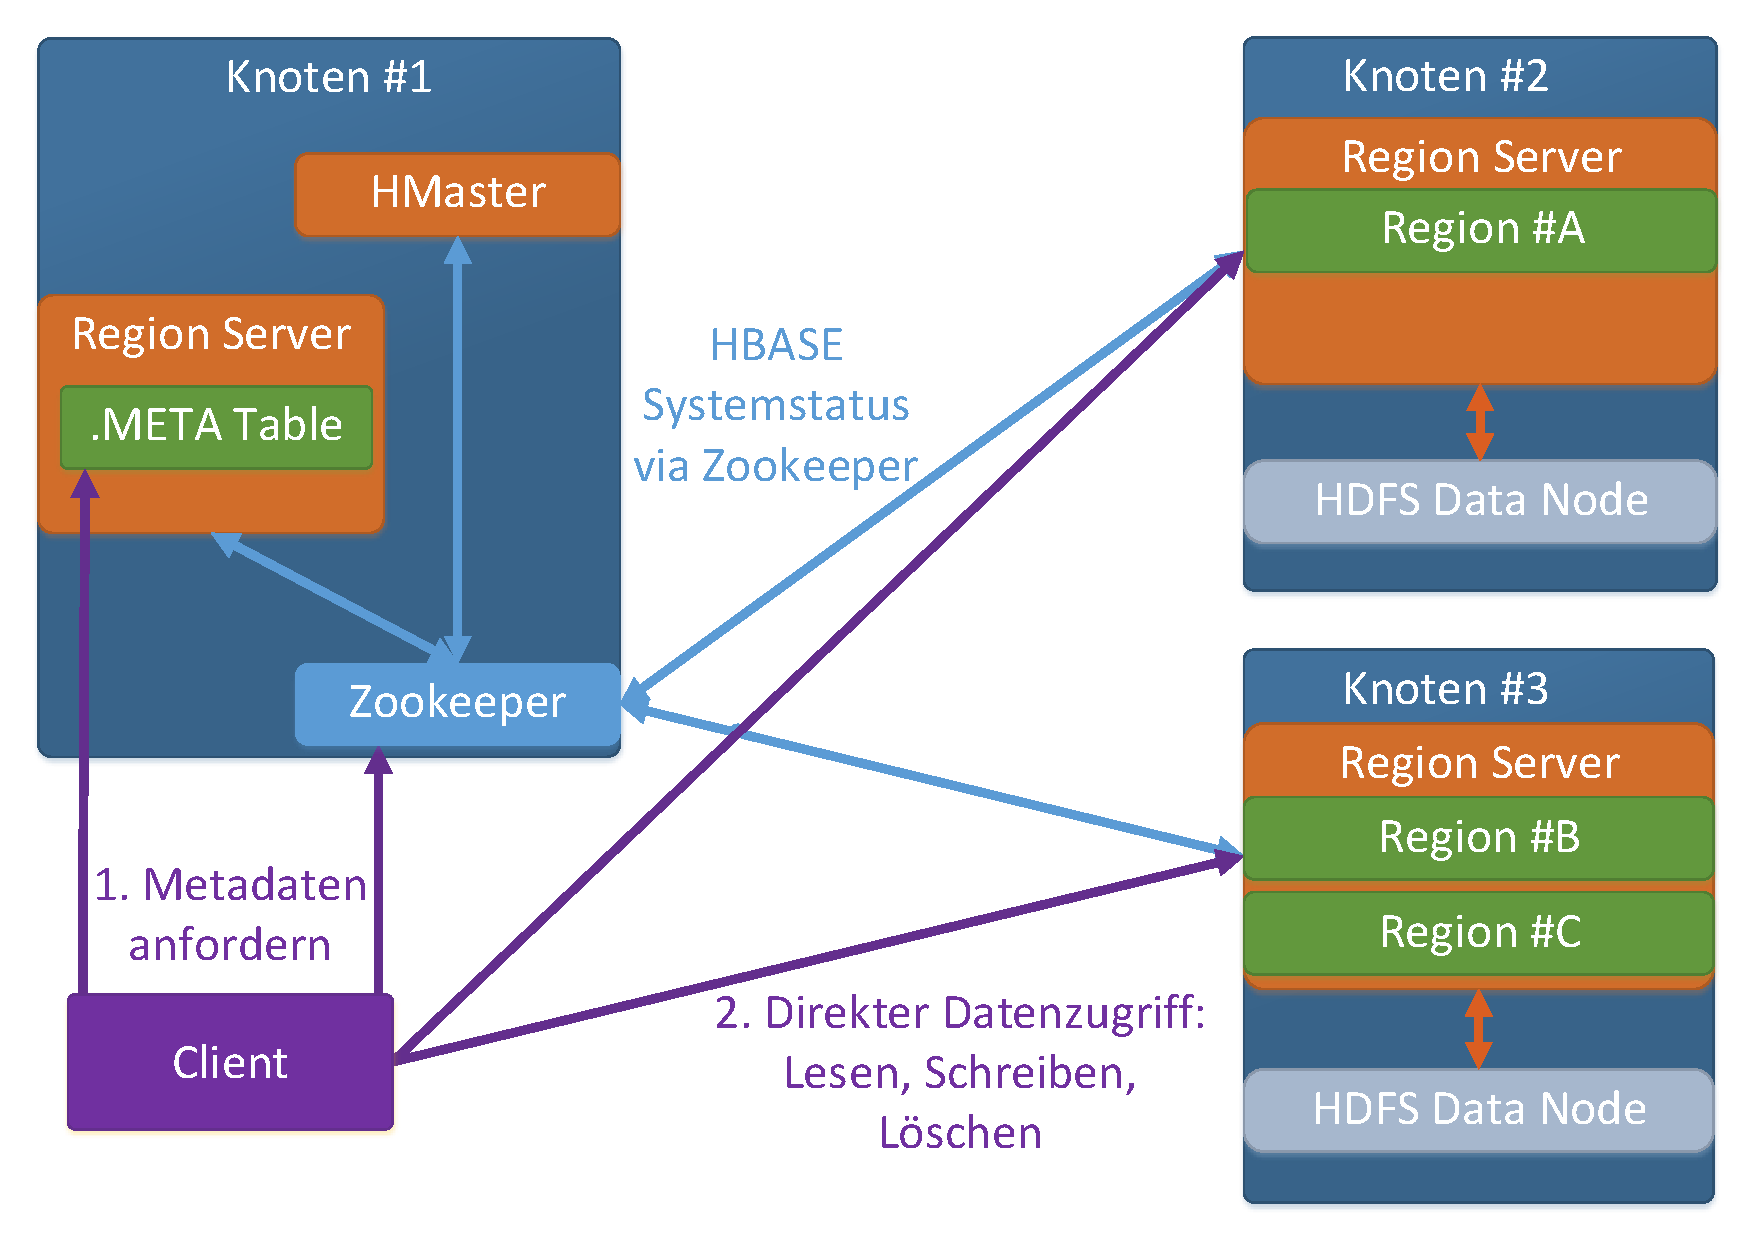
\includegraphics[width=\textwidth]{./resource/hbase_cluster_architecture.pdf}
  \caption{HBase Datenspeicherung im Cluster}
  \label{fig:hbase_cluster_architecture}
\end{figure}

\noindent
Auf den einzelnen Knoten im Computer-Cluster existieren sogenannte \textit{Region Server}. Diese Region Server speichern jeweils unterschiedliche Teile der angelegten HBase-Tabellen. 
Eine Tabelle wird hierbei anhand der Zeilenschlüssel in mehrere Bereiche, den sogenannten \textit{Regions}, unterteilt. Beispielsweise könnte die Region A die Daten einer Tabelle der Zeilen 1 bis 3.000 enthalten (siehe Abbildung \ref{fig:hbase_cluster_architecture}). Die Region B wiederum enthält die Daten von den Zeilen 3.001 bis 8.540 der gleichen Tabelle. Und die Region C könnte die Daten der Zeilen 1 bis 22.300 von einer anderen Tabelle enthalten. Somit kann ein Region Server mehrere Regions von gleichen oder auch unterschiedlichen Tabellen verwalten.  Das Prinzip der Datenlokalität greift auch bei HBase. So sollte auf  jedem Knoten, auf dem ein Region Server läuft, auch ein \gls{hdfs} Data Node existieren. Dieser speichert die Daten der einzelnen Regions als Dateien im \gls{hdfs}.\\

\noindent
Wenn neue Tabellen erstellt werden, oder einzelne Regions zu groß werden, dann koordiniert eine übergeordnete Instanz die Umverteilung von Daten und die Erstellung neuer Regions. Diese Instanz ist bei HBase der sogenannte \textit{HMaster}. Es ist ein unabhängiger Prozess, welcher auf einem beliebigen Knoten im Cluster läuft und über Apache ZooKeeper den Status der Region Server überwacht.\footnote{Die Funktionsweise von Apache ZooKeeper wird in Kapitel \ref{sec:theory_zookeeper} näher erläutert.} Um die Ausfallsicherheit zu gewährleisten, ist der Prozess redundant ausgelegt.\footnote{Über ZooKeeper kann der primäre HMaster-Prozess ermittelt werden. Ist der aktive HMaster nicht mehr erreichbar, schaltet sich ein Backup-HMaster ein.} Darüber hinaus kümmert sich der HMaster-Prozess auch um die Restrukturierung bei Teilausfällen einzelner Region Server.
Wenn nun ein Client auf die Daten einer Tabelle zugreifen möchte, muss dieser wissen, auf welchem Knoten die Daten abgelegt sind. Hierfür verbindet sich der Client zuerst mit ZooKeeper und erfährt darüber, welcher Region Server die sogenannte \textit{Meta-Tabelle} speichert.\cite[S. 579]{hadoop_definitive_guide}\\
Diese Meta-Tabelle enthält Informationen über alle HBase-Tabellen und der Region Server, welche die Regions bereitstellen. Anhand der Metadaten kann der Client die benötigten Daten direkt von den zuständigen Region Servern anfordern.
Dieses Vorgehen ist für den sporadischen Zugriff auf einzelne Datensätze nicht wirklich effizient. Es skaliert aber sehr gut bei großen Datenmengen, da kein Flaschenhals vorhanden ist. Üblicherweise speichert der Client die angeforderte Meta-Tabelle temporär ab, so dass er bei nachfolgenden Anfragen direkt auf die entsprechenden Region Server zugreifen kann.\\ 

\noindent
Im Rahmen der Thesis wird HBase verwendet, um Metadaten zu speichern. Diese werden wiederum mit Apache Spark ausgelesen und verarbeitet. Hierbei kann das Prinzip der Datenlokalität sehr gut genutzt werden.\\
In der Theorie ist es durchaus möglich, die HDFS Data Nodes, die Spark Worker und die HBase Region Server getrennt auf unterschiedlichen Knoten auszuführen. Dies ist aber nicht sinnvoll, da dadurch die Daten über das Netzwerk transportiert werden und die Verarbeitungsgeschwindigkeit verringert wird.\\
Sinnvoller ist es, die HDFS Data Nodes auf den Knoten auszuführen, wo auch die Region Server ausgeführt werden. Darauf aufbauend sollten auch die Spark Worker auf den Knoten gestartet werden, auf welchen die Region Server laufen. Dadurch können die Daten, welche von Apache Spark benötigt werden, direkt von dem lokalen HBase Region Server bereitgestellt werden. Dieser erhält die Daten wiederum von dem lokalen Data Node. Somit können die Daten direkt auf dem Knoten verarbeitet werden, wo sie auch gespeichert sind und müssen nicht über das Netzwerk an andere Knoten gesendet werden.\footnote{Siehe auch Kapitel \ref{sec:theory_yarn} und Kapitel \ref{sec:theory_spark}.} Die Koordinierung dieser Komponenten ist allerdings entsprechend komplex. Schon bei der Entwicklung von Anwendungen, können einzelne Fehler beim Datenzugriff dieses Prinzip der Datenlokalität aushebeln. Daher müssen die Anwendungen genau untersucht werden, ob sie das Prinzip der Datenlokalität korrekt umsetzen.\\

\section{Apache ZooKeeper}
\label{sec:theory_zookeeper}

Innerhalb eines Computer-Clusters zur verteilten Datenverarbeitung existiert oftmals das Problem, dass sich die einzelnen Komponenten koordinieren müssen. Beispielsweise teilt HBase die Daten auf mehrere Region Server auf, welche wiederum auf den einzelnen Knoten ausgeführt werden. Doch welche Instanz koordiniert diese Aufteilung? Ein anderes Problem ist der Datenzugriff. Ein Client möchte eine Zeile einer bestimmten Tabelle auslesen. Woher weiß der Client, welchen konkreten Knoten er anfragen muss, um genau diese Zeile zu erhalten?\\ 

\noindent
In den meisten Fällen existiert hierzu eine bestimmte Instanz, welche die Koordinierung der Knoten übernimmt. Bei HBase gibt es den HMaster-Prozess, der für diese Aufgaben verantwortlich ist. Das Problem dabei ist, dass auch der Knoten auf dem diese Master-Instanz läuft, ausfallen kann und das komplette System zum erliegen bringt. Diese Verwaltungsinstanzen im Allgemeinen, sind kritische Komponenten und können als Single-Point-of-Failure zu einem Stillstand des kompletten Systems führen. Um solche Totalausfälle zur vermeiden, müssen bestimmte Automatismen definiert werden, wie sich die Knoten selbst organisieren können, um einen Ausfall beliebiger Knoten zu überstehen.\\

\noindent
An dieser Stelle bietet \textit{Apache ZooKeeper\texttrademark\thinspace} Mechanismen an, wie sich die einzelnen Knoten in einem verteilten System organisieren und Informationen verteilt synchronisieren können. Aus logischer Sicht stellt ZooKeeper einen Service zu Verfügung. 
Dieser Service ermöglicht das Speichern von Informationen in einem strukturierten Verzeichnis mit einzelnen Dateien. Bei den Informationen handelt sich normalerweise um wichtige Konfigurationen, welche im Cluster verteilt werden müssen und zentral über ZooKeeper aktualisiert werden können. Jeder Client, der sich mit ZooKeeper innerhalb des Computer-Clusters verbindet, sieht die gleiche Konfiguration und kann bei Bedarf auch bestimmte Konfigurationen ändern.\cite[S. 4-5]{professional_hadoop} \\
Aus Sicht des Entwicklers, stellt dieser Service die aktuellen Informationen im Cluster zur Verfügung. Wie der Service dies bewerkstelligt, ist ein Implementierungsdetail. 
Neben dem bereits erwähnten Konfigurationsmanagement, bietet ZooKeeper einen Naming-Service an oder ermöglicht es auch den Live-Status einzelner Knoten zu überwachen.\cite{zookeeper_essentials}\\

\noindent
Wie bei HBase in Kapitel \ref{sec:theory_hbase} bereits erwähnt wird, kann sich ein Client mit ZooKeeper verbinden und erhält darüber den aktuellen Knoten, auf welchem der HMaster-Prozess läuft. Darüber kann er die Metadaten zu allen Tabellen abfragen. Ein anderes Beispiel zeigt die Backup-Instanz des HMaster-Prozesses.
Dieser prüft über ZooKeeper den Status des primären HMaster-Prozesses und wird informiert, wenn letzterer nicht mehr verfügbar ist. Daraufhin propagiert sich die Backup-Instanz als neuen HMaster-Prozess im Cluster, um so die Funktionsfähigkeit von HBase aufrecht zu erhalten. Abbildung \ref{fig:zookeeper_dir} zeigt die Verzeichnisstruktur, welche stark an ein Verzeichnis eines Dateisystems erinnert. Die einzelnen Einträge werden \textit{ZNodes} genannt.\footnote{Siehe Link \url{http://zookeeper.apache.org/doc/r3.5.4-beta/zookeeperOver.html}. Letzter Zugriff: 26.7.2018.} \\

\begin{figure}[ht]
  \centering
  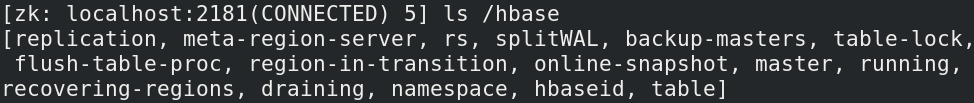
\includegraphics[width=\textwidth]{./resource/zookeeper_dir.png}
  \caption{Gespeicherte Informationen von HBase in ZooKeeper}
  \label{fig:zookeeper_dir}
\end{figure}


\noindent
Normalerweise ist ZooKeeper auf mehreren Knoten im Cluster installiert. Sie bilden ein sogenanntes \textit{ZooKeeper Ensemble} und bestehen zumeist aus 3 oder 5 Einzelinstallationen auf beliebigen Knoten. Ein ZooKeeper Ensemble, welches für die gleiche Anwendungsdomäne zuständig ist, wird auch \textit{Quorum} genannt. Innerhalb eines Quorums gibt es einen Leader und mehrere Follower, die sich die gleichen Konfigurationsinformationen teilen. Fällt der Leader aus, können die Follower selbstständig einen neuen Leader bestimmen.\cite{zookeeper_essentials}\\

\section{Apache Solr und Lucene}
\label{sec:theory_solr}
\textit{Apache Solr\texttrademark\thinspace} ist eine skalierbare und performante Plattform zur Volltextsuche. Die Daten werden vorher indexiert und können effizient durchsucht werden.\cite{solr_search} Mithilfe von Apache Solr werden zum Beispiel Volltextsuchen für Dokumente oder Produktsuchen für Webshops implementiert.

\noindent
Im Allgemeinen ist ein Suchsystem in mehrere Analyseschritte aufgeteilt. Ein Großteil dieser Verarbeitungsschritte wird nicht von Solr selbst übernommen. Vielmehr baut Solr auf dem Open-Source Projekt \textit{Apache Lucene\texttrademark\thinspace} auf und erweitert letzteres um eine skalierbare Infrastruktur und diverse Schnittstellen zur Verarbeitung der Daten.\\
Zu Beginn liegen beliebige Daten in Form von Dateien oder Dokumenten vor. Diese Daten durchlaufen eine textuelle Aufbereitung, bevor sie indexiert werden können.\\ 
Bei der Textanalyse wird der relevante Text aus den Daten extrahiert. Hierbei hängt die Extraktion der Daten auch davon ab, ob die Daten strukturiert, semistrukturiert oder unstrukturiert sind. Anhand der Dateiformate können diverse Bibliotheken genutzt werden, um Daten zu extrahieren. Beispielsweise kann mithilfe von \textit{Apache PDFBox\textsuperscript{\textregistered}}\footnote{Siehe Link: \url{https://pdfbox.apache.org/}. Letzter Zugriff: 01.08.2018.} Text aus \acrshort{pdf}-Dokumenten extrahiert werden. Mithilfe der \textit{\gls{gdal}}\footnote{Siehe Link: \url{https://www.gdal.org/}. Letzter Zugriff: 01.08.2018.} können Geopositionen aus den \acrshort{exif}-Metadaten von \acrshort{jpeg}-Bildern extrahiert werden. Mithilfe von \textit{Tesseract \acrshort{ocr}}\footnote{Siehe Link: \url{https://github.com/tesseract-ocr/tesseract}. Letzter Zugriff: 01.08.2018.} kann lesbarer Text direkt aus Bildern extrahiert werden.\cite[S. 39]{solr_search}\\

\noindent
Im nächsten Schritt wird der extrahierte Text aufbereitet. Die Aufbereitung hängt stark von dem spezifischen Anwendungsfall und den Daten ab. Im Allgemeinen werden Satzzeichen und überflüssige Füllwörter entfernt und Großbuchstaben werden in Kleinbuchstaben umgewandelt. Darüber hinaus kann auch eine Stammformreduktion durchgeführt werden. Darauf aufbauend kann der Text detaillierter analysiert werden. Beispielsweise könnten Redewendungen erkannt oder Synonyme einzelner Wörter identifiziert werden.\cite[S.44]{solr_search}\\

\noindent
Nach der Aufbereitung des Textes, erfolgt die Erstellung eines sogenannten \textit{Inverted Indexes}. Ein Inverted Index ist ähnlich aufgebaut wie ein Stichwortverzeichnis. Jedes Wort wird darin mit den Verweisen zu den Vorkommen in den einzelnen Dokumenten versehen. Auf Basis dieses Indexes können sehr schnell alle Dokumente gefunden werden, welche das gesuchte Wort enthalten.\cite[S. 47]{solr_search}\\

\noindent
Auf die erstellten Indizes können nun Suchanfragen durchgeführt werden. Aber auch hier gibt es unterschiedliche Modelle, wie die relevanten Dokumente ermittelt werden und in welcher Reihenfolge die Ergebnismenge zurückgeliefert wird.\\
Es gibt das sogenannte \textit{Boolean Model} auf Basis der booleschen Algebra. Beispielsweise könnte eine forensische Suchanfrage lauten: Suche alle Bilder oder Videos, welche das Wort \textit{Unfall} im Dateinamen haben, aber nicht kleiner als 1 MB groß sind. Diese Suchanfrage wird in einen booleschen Ausdruck überführt und die Dateien werden zurückgeliefert. Allerdings liefert dieses Modell keine Aussage zur Reihenfolge der Ergebnismenge.\\
Hierzu gibt es komplexere Suchmodelle, wie das sogenannte \textit{Vector Space Model}. Es basiert auf gewichteten Faktoren und ermöglicht es, für jedes Dokument der Ergebnismenge die Trefferwahrscheinlichkeit zu ermitteln. Nach dieser Bewertung wird die Reihenfolge der Ergebnisse festgelegt. Beispielsweise sollte ein Dokument eine höhere Bewertung erhalten, wenn das gesuchte Wort mehrfach im Dokument vorhanden ist.\cite[S. 47 ff.]{solr_search}\\

\noindent
Solr besitzt einen \textit{Cloud-Mode}, der es erlaubt, die indexierten Daten verteilt auf mehreren Knoten zu speichern. Dieser Cloud-Mode ist für eine Integration in das Hadoop-Ökosystem optimal.\footnote{Der Cloud-Mode kann aber auch ohne Apache Hadoop auf einem beliebigen Cluster genutzt werden.} Abbildung \ref{fig:solr_cluster_architecture} skizziert diese Verteilung im Computer-Cluster.\\

\begin{figure}[ht]
  \centering
  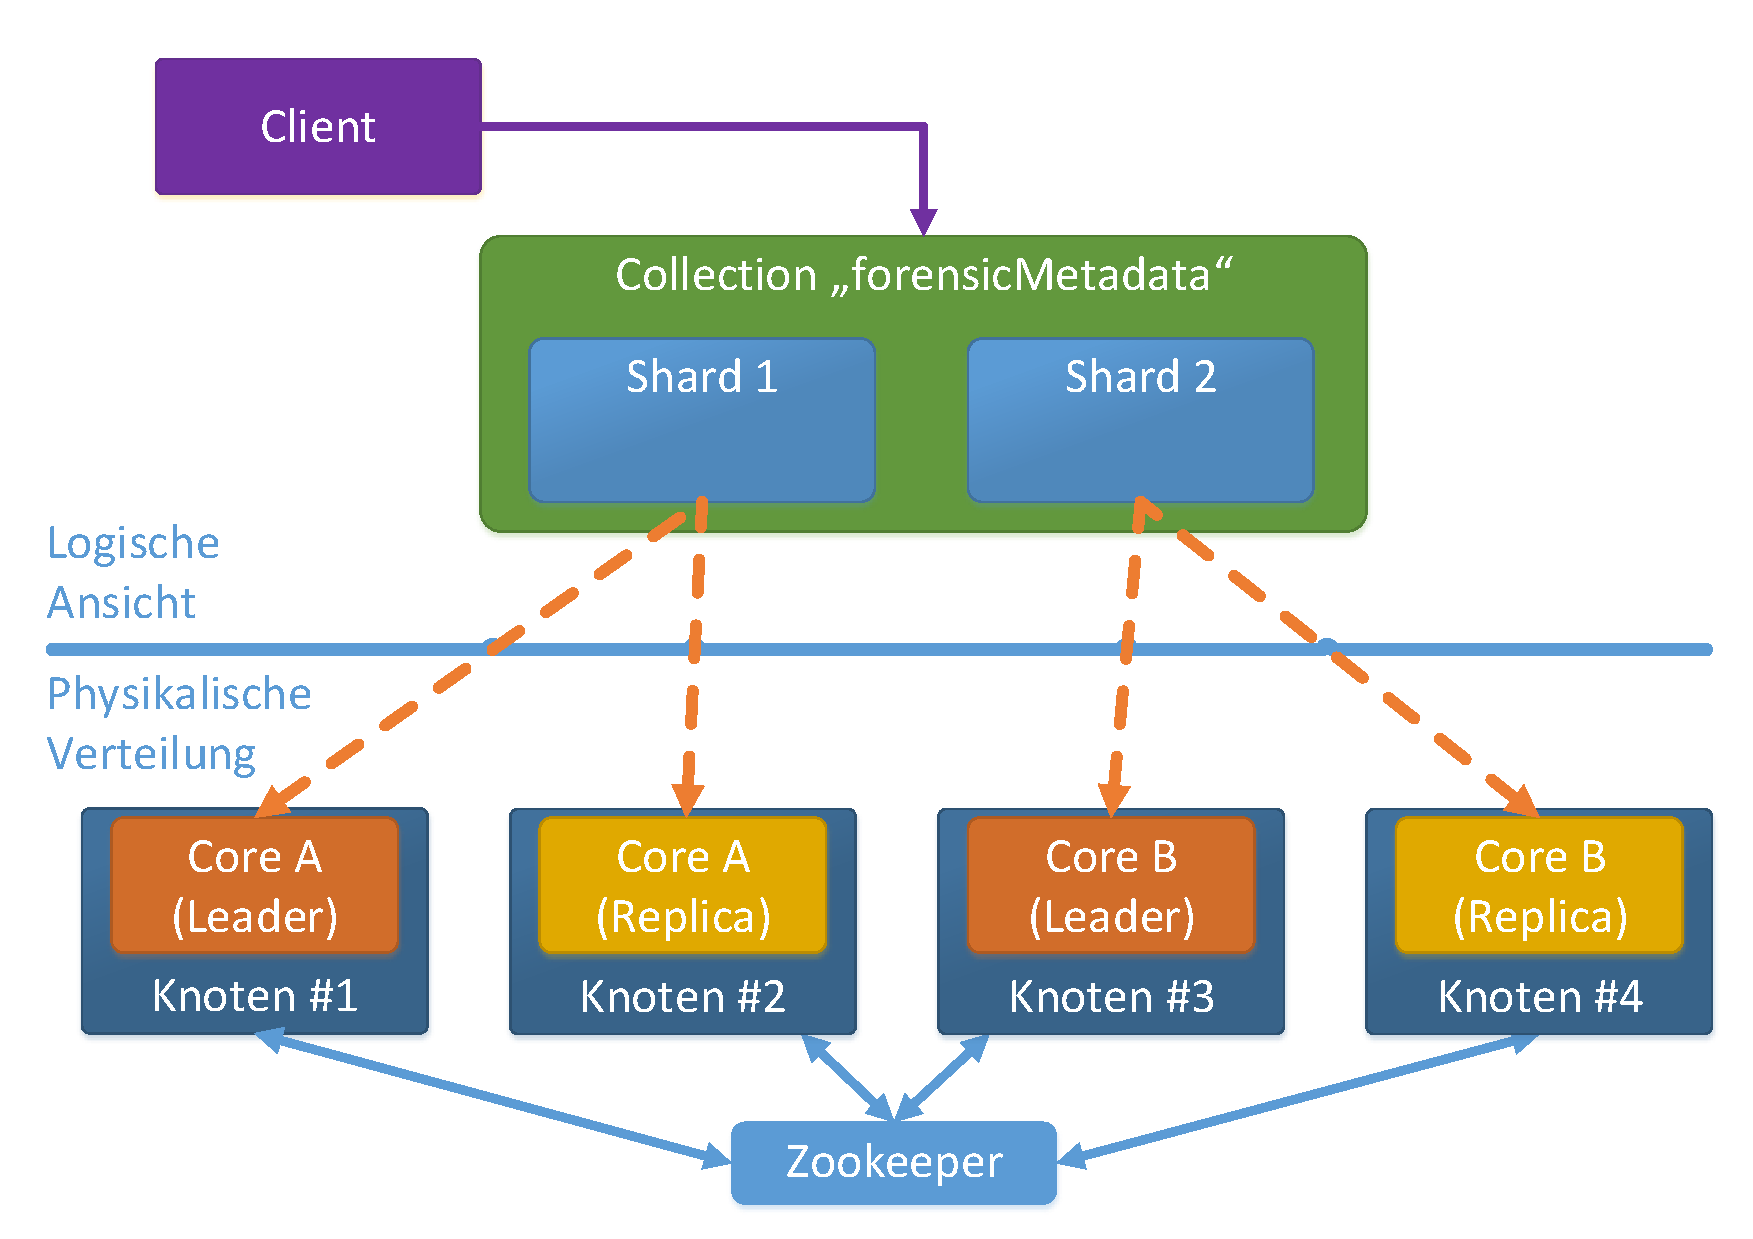
\includegraphics[width=\textwidth]{./resource/solr_cluster_architecture.pdf}
  \caption{Solr Cloud-Mode im Cluster}
  \label{fig:solr_cluster_architecture}
\end{figure}

\noindent
Dieser Cloud-Mode wird auch bei der Integration in die Analyseplattform genutzt.\footnote{Siehe Kapitel \ref{subsec:file_indexing}.} Solr kann als zusätzliches Software-Paket in das Hadoop-Ökosystem integriert werden.\footnote{Die Hortonworks Dataplatform bietet ein passendes Software-Paket zur Installation von Solr an. Primär wird dieses Paket genutzt, um eine performante Suche im \gls{hdfs}-Dateisystem zu ermöglichen. Die Solr-Installation kann aber auch für andere Zwecke genutzt werden.} Es können beliebige Daten in der Solr-Cloud indexiert werden. 
Darüber hinaus nutzt Solr im Cloud-Mode das bereits beschriebene ZooKeeper-Projekt\footnote{Siehe Kapitel \ref{sec:theory_zookeeper}.} zur Koordinierung und Überwachung der einzelnen Knoten.\\
Innerhalb des Cloud-Modes werden die oben beschriebenen Indizes (Inverted Index) in mehrere sogenannte \textit{Shards} aufgeteilt. Ein einzelner Shard ist ein Teil des Indexes, welcher unabhängig von den anderen Shards durchsucht werden kann. So werden bei einer Suchanfrage alle Shards parallel durchsucht. Einzelne Shards können wiederum auf anderen Knoten repliziert werden, um die Ausfallsicherheit zu gewährleisten. Solr spricht hierbei von Cores. Ein Core ist die physikalische Repräsentation eines logischen Shards auf einem konkreten Knoten. Alle logischen Shards bilden zusammen den Index, welcher bei Solr als sogenannte \textit{Collection} dargestellt wird.\cite{solr_cloud_scaling}\\

\noindent
Jedes Dokument, das in einer Collection indexiert werden soll, wird einem der logischen Shards zugeteilt. Hierbei wird zuerst anhand eines eindeutigen Dokumentenschlüssels entschieden, in welchen Shard das Dokument aufgenommen werden soll.\footnote{Der Dokumentenschlüssel kann zum Beispiel von der Hashsumme der Datei abgeleitet werden.} Ein logischer Shard wird abermals aufgeteilt in mehrere Replicas, den bereits erwähnten Cores auf den einzeln Knoten. 
Für jeden logischen Shard wird ein \textit{Leader}-Knoten bestimmt.\footnote{Diese Leader werden mittels ZooKeeper im Cluster propagiert.} Der Leader speichert einen physikalischen Core des logischen Shards und indexiert eingehende Dokumente. Sobald der Index für diesen Shard neu aufgebaut wurde, wird die Aktualisierung an die Knoten weitergesendet, die eine Replica (Core) des gleichen logischen Shards speichern.\cite[S. 867-872]{solr_ref_guide}\\ 


\noindent
Apache Solr und Lucene sind beide in Java implementiert. Daher gibt es einen Java Client, zur Durchführung von Suchanfragen. Andererseits existiert auch ein \gls{rest}-Endpunkt, der für Anfragen genutzt werden kann. Damit können Anfragen simpel und schnell in beliebige Websites integriert werden oder direkt mit dem Kommandozeilentool \textit{curl} durchgeführt werden. Hierbei können die Anfragen in \acrshort{xml} (\acrlong{xml}) oder \acrshort{json} (\acrlong{json}) formatiert sein. Ein simples Beispiel zeigt nachfolgende Anfrage (siehe Abbildung \ref{fig:solr_request}).\\

\begin{figure}[ht]
  \centering
  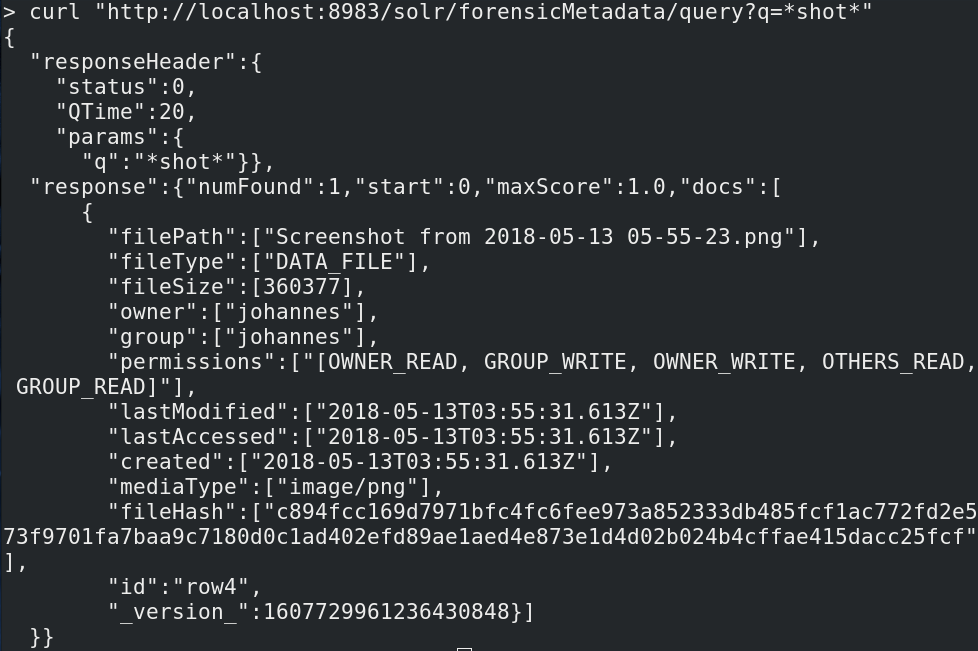
\includegraphics[width=\textwidth]{./resource/solr_request.png}
  \caption{Solr-Suchanfrage via \textit{curl}}
  \label{fig:solr_request}
\end{figure}

\noindent
In dem Beispiel ist die Solr-Instanz unter \url{http://localhost:8983} erreichbar. Die Suchanfrage wird auf der Collection \textit{forensicMetadata} ausgeführt. Es soll in allen Feldern nach einem Vorkommen von dem Wort \textit{shot} (\textit{q=*shot*}) gesucht werden. Die Antwort ist im JSON-Format definiert. Unter anderem wird die Anzahl der Treffer (\textit{numFound:1}) mitgeliefert. Bei dieser konkreten Anfrage, wurde ein Bild mit dem Dateinamen \textit{Screenshot...} gefunden. 